% **************************************************************************************************************
%
% **************************************************************************************************************
\documentclass[ twoside,openright,titlepage,numbers=noenddot,toc=bibliography,%
                footinclude=false,headinclude=false,cleardoublepage=empty,%
								DIV=15,BCOR=5mm,paper=a4,fontsize=11pt,%
                ngerman,%
               ]{scrreprt}

%***************************************************************************************************************
% Note: Make all your adjustments in here
%***************************************************************************************************************
% ****************************************************************************************************
% htwsaar-i-mst-config.tex 
% ****************************************************************************************************  
								
% ****************************************************************************************************
% 1. Personal data and user ad-hoc commands
% ****************************************************************************************************
\newcommand{\myTitle}{Zusammenfassung des TK-Praktikum des sechsten Semesters Kommunikationsinformatik}
\newcommand{\myDegree}{Praktikum\xspace}
%\newcommand{\myDegree}{Master-Thesis\xspace}
\newcommand{\myName}{Deniz Kadiogullari und Christoph Drost\xspace}
\newcommand{\myUni}{htw saar -- Hochschule f�r Technik und Wirtschaft des Saarlandes\xspace}
\newcommand{\myCompany}{\xspace}
\newcommand{\myFirstProf}{Harald Krauss\xspace}
\newcommand{\mySecondProf}{Horst Wieker\xspace}
\newcommand{\myLocation}{Saarbr�cken\xspace}
\newcommand{\myTime}{20.~Mai~2014\xspace}
\newcommand{\currentVersion}{Version 1.0\xspace} % TODO: ggf. �ber git Versionsinformationen automatisch bereitstellen und verwenden

% ********************************************************************
% Setup, finetuning, and useful commands
% ********************************************************************
\newcounter{dummy} % necessary for correct hyperlinks (to index, bib, etc.)
% ****************************************************************************************************


% ****************************************************************************************************
% 2. Loading some handy packages
% ****************************************************************************************************
% ******************************************************************** 
% Packages with options that might require adjustments
% ******************************************************************** 
\PassOptionsToPackage{latin9}{inputenc}	% latin9 (ISO-8859-9) = latin1+"Euro sign"
 \usepackage{inputenc}				

\PassOptionsToPackage{ngerman}{babel}   % change this to your language(s)
 \usepackage{babel}					
 \usepackage{csquotes}
	
\PassOptionsToPackage{language=auto,style=numeric-comp,backend=bibtex8,maxbibnames=50}{biblatex}
 \usepackage{biblatex}	
 \bibliography{quellen}			

\PassOptionsToPackage{fleqn}{amsmath}		% math environments and more by the AMS 
 \usepackage{amsmath}

% ******************************************************************** 
% Setting up the page and margins
% ******************************************************************** 
\usepackage{geometry}
%\geometry{a4paper,left=20mm,right=20mm,top=25mm,bottom=30mm}

% ******************************************************************** 
% General useful packages
% ******************************************************************** 
\PassOptionsToPackage{T1}{fontenc} % T2A for cyrillics
\usepackage{fontenc}  
%\usepackage[automark]{scrpage2}
\PassOptionsToPackage{dvipsnames}{xcolor}
	\RequirePackage{xcolor} % [dvipsnames]  
	\definecolor{ingwi}{cmyk}{.9,0,0,0}
\usepackage{textcomp} % fix warning with missing font shapes
\usepackage{scrhack} % fix warnings when using KOMA with listings package          
\usepackage{xspace} % to get the spacing after macros right  
\usepackage{mparhack} % get marginpar right
\usepackage{fixltx2e} % fixes some LaTeX stuff 
\PassOptionsToPackage{printonlyused}{acronym}
	\usepackage{acronym} % nice macros for handling all acronyms in the thesis
\renewcommand{\bflabel}[1]{{#1}\hfill} % fix the list of acronyms
\usepackage{booktabs}
\usepackage{multirow}
\usepackage[shadow]{todonotes} %Settings for ToDoNotes
% Eigene Shortcuts fuer laengere Befehle
	\newcommand{\todox}[1]{\todo[inline, size=\small]{#1}}
	%Nummerierte Anmerkungen
	\newcounter{todocounter}
	\renewcommand{\todox}[2][]{\stepcounter{todocounter}\todo[inline, size=\small,caption={\thetodocounter: #2}, #1]{\renewcommand{\baselinestretch}{0.5}\selectfont\thetodocounter: #2\par}}
\usepackage{blindtext}
%\usepackage{footmisc}
% ****************************************************************************************************


% ****************************************************************************************************
% 3. Setup floats: tables, (sub)figures, and captions
% ****************************************************************************************************
\usepackage{tabularx} % better tables
	\setlength{\extrarowheight}{3pt} % increase table row height
%\newcommand{\myfloatalign}{\centering} % to be used with each float for alignment
\usepackage{caption}
\captionsetup{format=hang,font=small}
\usepackage{subfig}
\usepackage{wrapfig}
% ****************************************************************************************************


% ****************************************************************************************************
% 6. Setup code listings
% ****************************************************************************************************
\usepackage{listings} 
%\lstset{emph={trueIndex,root},emphstyle=\color{BlueViolet}}%\underbar} % for special keywords
\lstset{language=[LaTeX]Tex,%C++,
    keywordstyle=\color{RoyalBlue},%\bfseries,
    basicstyle=\small\ttfamily,
    %identifierstyle=\color{NavyBlue},
    commentstyle=\color{Green}\ttfamily,
    stringstyle=\rmfamily,
    numbers=none,%left,%
    numberstyle=\scriptsize,%\tiny
    stepnumber=5,
    numbersep=8pt,
    showstringspaces=false,
    breaklines=true,
    frameround=ftff,
    frame=single,
    belowcaptionskip=.75\baselineskip
    %frame=L
} 
%Styles f�r verschiedene Sprachen festlegen, z.B. Java
\lstdefinestyle{Java}{
belowcaptionskip=1\baselineskip,
  breaklines=true,
  xleftmargin=\parindent,
  language=Java,
  showstringspaces=false,
  basicstyle=\footnotesize\ttfamily,
  keywordstyle=\bfseries\color{green!40!black},
  commentstyle=\itshape\color{purple!40!black},
  identifierstyle=\color{blue},
  stringstyle=\color{orange}}
% ****************************************************************************************************    		   


% ****************************************************************************************************
% 6. PDFLaTeX, hyperreferences and citation backreferences
% ****************************************************************************************************
% ********************************************************************
% Using PDFLaTeX
% ********************************************************************
\PassOptionsToPackage{pdftex,hyperfootnotes=false,pdfpagelabels}{hyperref}
	\usepackage{hyperref}  % backref linktocpage pagebackref
\pdfcompresslevel=9
\pdfadjustspacing=1 
\PassOptionsToPackage{pdftex}{graphicx}
	\usepackage{graphicx} 
    

% ********************************************************************
% Hyperreferences
% ********************************************************************
\hypersetup{%
    %draft,	% = no hyperlinking at all (useful in b/w printouts)
    pdfstartpage=1, pdfstartview=FitV,%
		colorlinks=true, linktocpage=true,
		%urlcolor=Black, linkcolor=Black, citecolor=Black, %pagecolor=Black,%
		%urlcolor=brown, linkcolor=RoyalBlue, citecolor=green, %pagecolor=RoyalBlue,%
    % uncomment the following line if you want to have black links (e.g., for printing)
    %colorlinks=false, pdfborder={0 0 0},
    breaklinks=true, pdfpagemode=UseNone, pageanchor=true, pdfpagemode=UseOutlines,%
    plainpages=false, bookmarksnumbered, bookmarksopen=true, bookmarksopenlevel=1,%
    hypertexnames=true, pdfhighlight=/O,%nesting=true,%frenchlinks,%
    pdftitle={\myTitle},%
    pdfauthor={\textcopyright\ \myName, \myUni},%
    pdfsubject={},%
    pdfkeywords={},%
    pdfcreator={pdfLaTeX},%
    pdfproducer={LaTeX with hyperref}%
}   

% ********************************************************************
% Setup autoreferences
% ********************************************************************
% There are some issues regarding autorefnames
% http://www.ureader.de/msg/136221647.aspx
% http://www.tex.ac.uk/cgi-bin/texfaq2html?label=latexwords
% you have to redefine the makros for the 
% language you use, e.g., american, ngerman
% (as chosen when loading babel/AtBeginDocument)
% ********************************************************************
\makeatletter
\@ifpackageloaded{babel}%
    {%
       \addto\extrasamerican{%
					\renewcommand*{\figureautorefname}{Figure}%
					\renewcommand*{\tableautorefname}{Table}%
					\renewcommand*{\partautorefname}{Part}%
					\renewcommand*{\chapterautorefname}{Chapter}%
					\renewcommand*{\sectionautorefname}{Section}%
					\renewcommand*{\subsectionautorefname}{Section}%
					\renewcommand*{\subsubsectionautorefname}{Section}% 	
				}%
       \addto\extrasngerman{% 
					\renewcommand*{\chapterautorefname}{Kapitel}%
					\renewcommand*{\sectionautorefname}{Abschnitt}%
					\renewcommand*{\subsectionautorefname}{Abschnitt}%
					\renewcommand*{\subsubsectionautorefname}{Abschnitt}% 
					\renewcommand*{\paragraphautorefname}{Absatz}%
					\renewcommand*{\subparagraphautorefname}{Absatz}%
					\renewcommand*{\footnoteautorefname}{Fu\"snote}%
					\renewcommand*{\FancyVerbLineautorefname}{Zeile}%
					\renewcommand*{\theoremautorefname}{Theorem}%
					\renewcommand*{\appendixautorefname}{Anhang}%
					\renewcommand*{\equationautorefname}{Gleichung}%        
					\renewcommand*{\itemautorefname}{Punkt}%
				}%	
			% Fix to getting autorefs for subfigures right (thanks to Belinda Vogt for changing the definition)
			\providecommand{\subfigureautorefname}{\figureautorefname}%  			
    }{\relax}
\makeatother


% ****************************************************************************************************
% 6. Last calls before the bar closes
% ****************************************************************************************************
% ********************************************************************
% Development Stuff
% ********************************************************************
%\listfiles
\PassOptionsToPackage{l2tabu,orthodox,abort}{nag}
	\usepackage{nag}
%\PassOptionsToPackage{warning, all}{onlyamsmath}
%	\usepackage{onlyamsmath}


% ****************************************************************************************************
% 7. Further adjustments (experimental)
% ****************************************************************************************************
\usepackage{tocbibind} %Allows us to add Bibliography to ToC
% ********************************************************************
% Using different fonts
% ********************************************************************
%\usepackage[oldstylenums]{kpfonts} % oldstyle notextcomp
%\usepackage[osf]{libertine}
%\usepackage{hfoldsty} % Computer Modern with osf
%\usepackage[light,condensed,math]{iwona}
%\renewcommand{\sfdefault}{iwona}
%\usepackage{lmodern} % <-- no osf support :-(
\usepackage{mathpazo} 
%\usepackage[urw-garamond]{mathdesign} <-- no osf support :-(

\setkomafont{disposition}{\bfseries}
% ****************************************************************************************************

\usepackage{framed}  %Fuer boxen mit Textumbruch
\usepackage{diagbox} % Um eine diagonale Linie in Tabellen zu ziehen

\usepackage{float} %Vereinfacht die Positionierung von Float Umgebungen(Bild, Tabelle...)
%********************************************************************
% Hyphenation
%*******************************************************
%\hyphenation{put special hyphenation here}

% ********************************************************************
% GO!GO!GO! MOVE IT!
%*******************************************************
\begin{document}
\frenchspacing
\raggedbottom
\selectlanguage{ngerman} % american ngerman
\pagenumbering{roman}
\pagestyle{plain}
%********************************************************************
% Frontmatter
%*******************************************************
%*******************************************************
% Titlepage
%*******************************************************
\begin{titlepage}

\includegraphics[width=\linewidth]{Graphics/htwsaar_Logo_inwi_head_VF_4C_crop}
  \begin{center}
    \large  
    \hfill
    \vfill
    \begingroup
      \Large\bfseries\myTitle \\ \bigskip
    \endgroup

  \myDegree %\\ \bigskip

  \vfill
  \myName
  \vfill
  Erstgutachter: \myFirstProf \\
  Zweitgutachter: \mySecondProf \\ % Zweitgutachter idR nur bei Master-Arbeiten
  Einreichung: \myTime
%\vfill                      

    \end{center}       
\end{titlepage}   
\clearpage%*******************************************************
% Abstract
%*******************************************************
%\pdfbookmark[0]{Zusammenfassung}{Zusammenfassung}
\chapter*{Zusammenfassung}
Kurze Zusammenfassung des Inhaltes in deutscher Sprache, der Umfang betr�gt zwischen einer halben und einer ganzen DIN A4-Seite.

Orientieren Sie sich bei der Aufteilung bzw. dem Inhalt Ihrer Zusammenfassung an Kent Becks Artikel: \url{http://plg.uwaterloo.ca/~migod/research/beckOOPSLA.html}.
\cleardoublepage%*******************************************************
% Table of Contents
%*******************************************************
\setcounter{tocdepth}{2} % <-- 2 includes up to subsections in the ToC
\setcounter{secnumdepth}{3} % <-- 3 numbers up to subsubsections

%\pdfbookmark[1]{\contentsname}{toc}
\tableofcontents 

\cleardoublepage
\begingroup
	\let\clearpage\relax
	\let\cleardoublepage\relax
	\listoffigures
	\listoftables
	\addcontentsline{toc}{chapter}{\lstlistlistingname}
	\lstlistoflistings 
	\chapter*{Abk�rzungsverzeichnis}
	\addcontentsline{toc}{chapter}{Abk�rzungsverzeichnis}	
	%Hier alle ben�tigten Abk�rzungen einf�gen
	\begin{acronym}[WLAN] % LONGEST ACRONYM HERE FOR CORRECT SPACING
	    \acro{WLAN}{Wireless Local Area Network}
	    \acro{TCP}{Transmission Control Protocol}
	    \acro{GoF}{Gang of Four}
	\end{acronym} %Abkuerzungsverzeichnis l�sst sich nicht ohne weiteres in ToC einbinden. Daher diese L�sung.
\endgroup                   


%********************************************************************
% Mainmatter
%*******************************************************
\pagenumbering{arabic}
\pagestyle{headings}
%\pagestyle{scrheadings}
\cleardoublepage
\include{tkinhalt/gsm}	 	% Diese Einbindungen werden nat�rlich entfernt, wenn es an die richtige
%=========================================
% 	   Einleitung     		 =
%=========================================

\chapter{BA Versuch}

\section{Allgemeine Beschreibung des Versuchs}
BA, Basic Access, ist der Standardanschluss an das ISDN Netz. Er wird von den Anbietern an Privatkunden und kleine Betriebe vergeben. Basic Access bietet zwei Nutzkan�le (B-Kan�le) und einen Signalisierungskanal (D-Kanal). Obwohl die Netzbetreiber nach und nach auf reine IP Netze umstellen, hat ISDN in �ffentlichen Telefonnetzen einen hohen Stellenwert. Mit der Entscheidung, dass die Ortsvermittlungsanlagen digitalisiert werden sollte, wurde 1979 ein wichtiger Grundstein f�r ISDN gelegt. 1987 wurde ISDN in Pilotprojekten erfolgreich getestet und schlie�lich 1989 fl�chendeckend eingef�hrt. ISDN bietet im Vergleich zu den analogen �bertragungstechniken den Vorteil, dass zwei Nutzkan�le gleichzeitig �bertragen werden k�nnen. Zus�tzliche Vorteile resultieren aus der verbesserten Sprachqualit�t und der schnelleren Daten�bertragung.

Der folgende Versuch soll das grundlegende Verst�ndnis f�r ISDN vertiefen und gleichzeitig Einblicke in die Konfiguration gew�hren. Der Einblick in die Konfiguration wird dadurch vermittelt, dass es zu dem Versuch geh�rt, die Anlage f�r den Versuch herzurichten. Durch Protokollmitschnitte und die bereitgestellten Unterlagen soll das grundlegende Verst�ndnis f�r ISDN vermittelt werden.

\section{Einrichten der Anlage}

\subsection{Einrichten der Ports \label{einrichtungPorts}}
\subsubsection{Aufbau des Versuchs}

Als Switch steht ein Patapsco Liberator S zur Verf�gung. Der Switch �bernimmt die Funktionen des Netzes. Dazu geh�ren die TEI Vergabe, das Routing von Gespr�chen und die Vergabe von Telefonnummern. Auf der Hardwareebene verbindet der Liberator die Telefone.

Zus�tzlich steht ein EyeSDN Ger�t zur Verf�gung. Dieses erm�glicht die Verbindung des Computers mit dem ISDN Netz und damit den Mittschnitt der Daten. 

Zur Telefonie stehen zwei Telefone zur Verf�gung und zum Konfigurieren des Systems ein Computer. Die Stromversorgung der Telefone wird vom Liberator eingespeist.

\subsubsection{Versuchsdurchf�hrung}
Die Hardware ist zu Beginn des Versuchs bereits verkabelt. Nachdem die SoftwareEyeSDN gestartet wurde, beginnt das Konfigurieren des Switches. Die Konfiguration des Switches geschieht in der Anwendung Switchmanager. Dort werden die Ports eingerichtet, an denen die Telefone h�ngen und die Freizeichen eingestellt. Nach dem Upload wird die Konfiguration auf den Switch �bertragen.

Die Einstellungen k�nnen direkt an den Telefonen getestet werden. Wenn der H�rer abgehoben wird, muss ein Freizeichen zu h�ren sein.


\subsubsection{}
\begin{figure}[htbp]
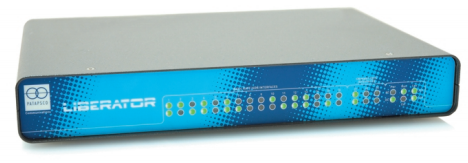
\includegraphics[width=0.7\textwidth]{tkinhalt/ba_bilder/liberator.png}
\caption{Der Loberator S \cite{liberatorBild}}
\label{darstellungLiberator}
\end{figure} 

\subsubsection{Auswertung des Versuchs}
Nachdem die Ports konfiguriert sind, und die Konfiguration auf den Liberator S �bertragen sind, sind die Telefone grunds�tzlich aktiv. Beide Telefone geben nach dem Abheben des H�rers ein Freizeichen. 

\subsection{Einrichten der Routing Tabellen}
Nach dem Versuch \ref{einrichtungPorts} haben die Telefone bereits Grundfunktionalit�ten. Zum Telefonieren und f�r die weiteren Versuche fehlt aber noch die Einrichtung der Routinginformationen. Ohne die Routinginformationen ist es nicht m�glich, ein Gespr�ch von einem Telefon zum Anderen zu leiten, also zu telefonieren.

\subsubsection{Aufbau des Versuchs}
Der Aufbau des Versuchs entspricht dem vom Versuch \ref{einrichtungPorts}. Dieser ist f�r den aktuellen Versuch aber eine Vorraussetzung.

\subsubsection{Beschreibung des Versuchs}
Das Routing wird im Interface Term des Liberator Fensters eingerichtet. F�r das Einrichten von  Routen k�nnen Profile angelegt werden, dadurch bleibt das System flexibler. Wir richten ein neues Profil ein, und konfigurieren die Routen von Telefon 1 zu Telefon 2  und umgekehrt. Wie bereits im letzten Versuch werden die Einstellungen nach dem Hochladen wirksam.

\subsubsection{Auswertung des Versuchs}
Nachdem die Routen konfiguriert sind, ist es m�glich das Telefon 2 vom Telefon 1 aus anzurufen. Ein Anruf in die Umgekehrte Richtung ist auch m�glich.

\section{Aufzeichnungen und Interpretationen des ISDN-D-Kanal Protokolls}
\subsection{Aufzeichnen des  ISDN-D-Kanal Protokolls \label{aufzeichnenDKanal}}
\subsubsection{Versuchsaufbau}
Der Versuchsaufbau entspricht dem Versuch  \ref{einrichtungPorts}. Die beiden vorangegangen Versuche sind f�r diesen voraus gesetzt.

\subsubsection{Versuchdurchf�hrung}
Die sp�tere Auswertung wird erleichtert, wenn der, eventuell schon laufende, Mitschnittsdienst erst gestoppt wird und alle vorhandenen Ergebnisse verworfen werden. Nachdem das geschehen ist, wird der Mitschnittdienst wieder gestartet und mit dem Telefon 1 das Telefon 2 angerufen. Wenn das Telefon 2 klingelt wird der H�rer abgehoben und nach einem kurzen Moment wieder aufgelegt. Dadurch wird ein Gespr�ch aufgebaut und wieder abgebaut. Direkt nach dem Beenden des Gespr�chs wird der Mitschnittdienst wieder gestoppt. 
Die Auswertung des Gespr�chs beginnt, wenn der Mitschnitt im Fenster mit einem Doppelklick ausgew�hlt wird. 

\subsection{Interpretieren des D-Kanal-Protokoll Mitschnitts}
\subsubsection{Versuchsaufbau}
Der Versuch \ref{aufzeichnenDKanal} muss durchgef�hrt sein und die Ergebnisse m�ssen vorliegen. F�r die Auswertung muss ein Computer mit der Software Wireshark bereit stehen.
\subsubsection{Versuchsdurchf�hrung}
Die aufgezeichneten Protokolldaten werden mit Wireshark ge�ffnet. 

\subsubsection{Auswertung des Versuchs}

\begin{figure}[H]
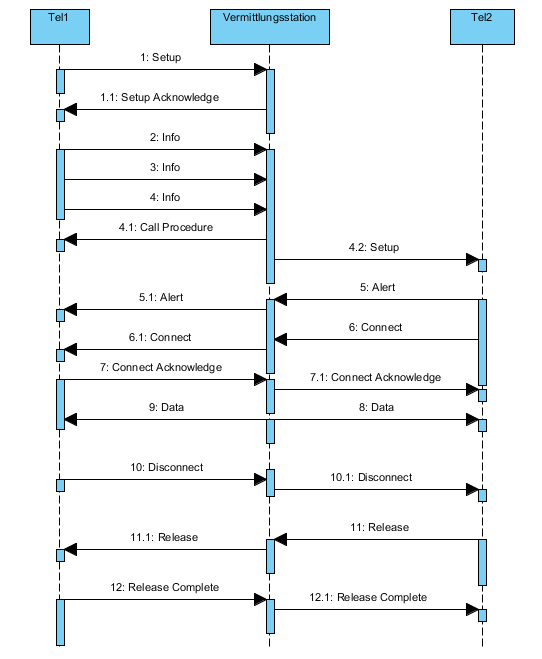
\includegraphics[width=0.8\textwidth]{tkinhalt/ba_bilder/diagramm_ba.png}
\caption{Aufbau und Abbau einer ISDN Verbindung}
\label{VerbindungISDN}
\end{figure}

Zur einfacheren und genaueren Auswertung des Versuchs sind in der Aufgabenbeschreibung 12 Fragen beschrieben. 
\begin{enumerate} 
	\item \textbf{Welche Rahmen dienen der TEI-Vergabe, und welcher TEI-Wert wird dem Telefon von der Vermittlung zugewiesen?} \newline
		Die TEI, Terminal Endpoint Identifier, Vergabe wird �ber das Protocol TEI mit der info Itenty Request behandelt. Diese fordert einen TEI Wert zur Indentifizierung des Endger�tes an. 
		
		\begin{figure}
		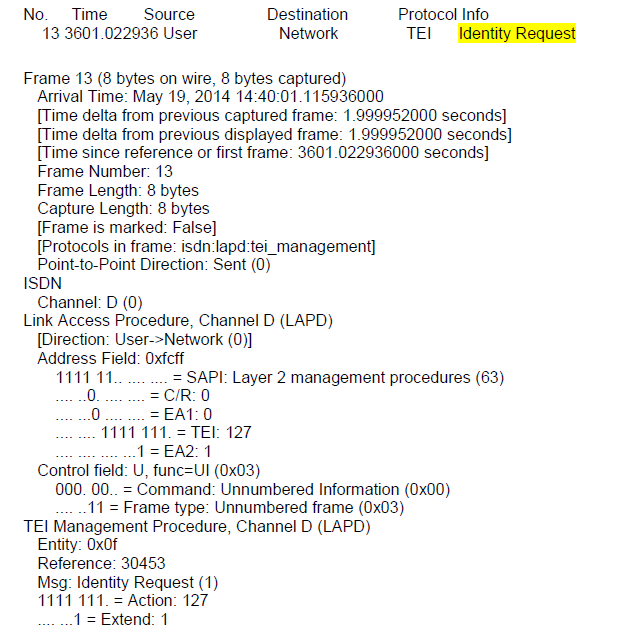
\includegraphics[width=0.8\textwidth]{tkinhalt/ba_bilder/ba/indenty_request_a1.png}
		\caption{Identy Request Frame}
		\label{identy_request_frame}
		\end{figure}
		
		Die Anfrage wird durch einen Identy Assigned best�tigt und ein TEI Wert wird dem Endger�t zugewiesen. In diesem Fall wird der Wert 64 zugewiesen.
		
		\begin{figure}
		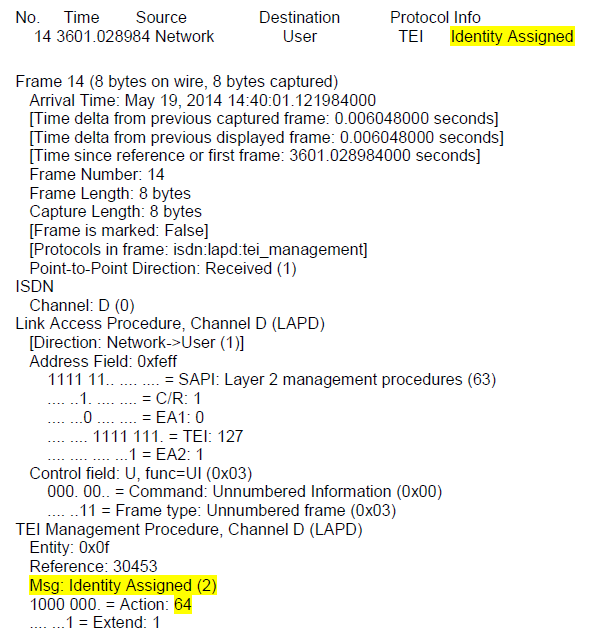
\includegraphics[width=0.8\textwidth]{tkinhalt/ba_bilder/ba/identy_assigned_a1.png}
		\caption{Identy Assigned Frame}
		\label{identy_assigned_frame}
		\end{figure}

	\item \textbf{Wann ist der Aufbau der Schicht 2 abgeschlossen?}  \newline
	Der Aufbau ist nach dem Senden eines unnumbered Acknowledge Frame beendet.  Dieser wird zur Best�tigung des Set Asynchronous Balance Mode Extended Frame benutzt.
		
		\begin{figure}[H]
		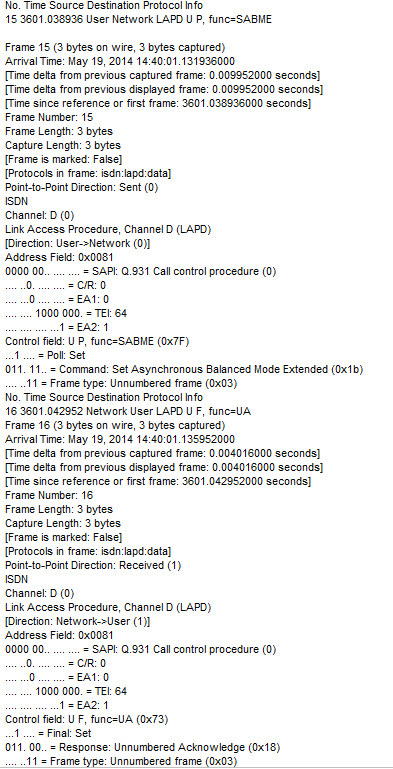
\includegraphics[width=0.8\textwidth]{tkinhalt/ba_bilder/ba/sabme_a2.png}
		\caption{SABME Nachricht}
		\label{sabme_nachricht}
		\end{figure}
	
	\item \textbf{Welchen ISDN-Dienst fordert das Telefon von der Vermittlungsstelle an, welche �bertragungskapazit�t ben�tigt dieser Dienst?}\newline
	Das Telefon fordert den Dienst zum �bertragen von Sprache an. Dies ist ein Kanal mit 64 kbit/s �bertragungskapazit�t.
	Im folgenden Frame kann man dies herauslesen. Es handelt sich hierbei um eine Setup Nachricht.
		
		\begin{figure}[H]
		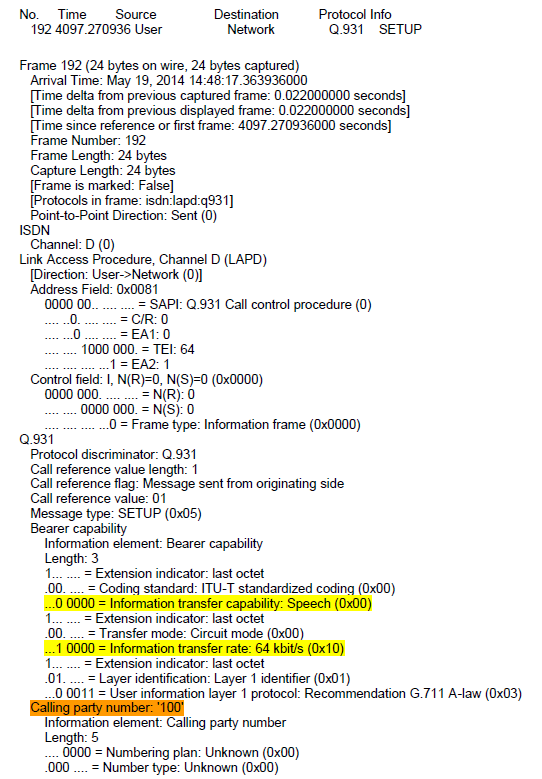
\includegraphics[width=0.8\textwidth]{tkinhalt/ba_bilder/ba/setup_a3.png}
		\caption{Setup Nachricht}
		\label{setup_nachricht}
		\end{figure}
	
	\item \textbf{Welche Kodierung des Sprachkanals wird gew�hlt?}\newline
		Wie man auf dem nachfolgenden Bild in Grau hinterlegt erkennen kann wird der TU-T Standardized-Coding verwendet.
		Diese Richtlinie gilt f�r das Digitalisieren analoger Audiosignale mittels Puls-Code-Modulation. Der Einsatzbereich f�r dieses Codecs ist, wie zu erwarten, in der klassischen sowie in der IP-Telefonie.
		\begin{figure}[H]
		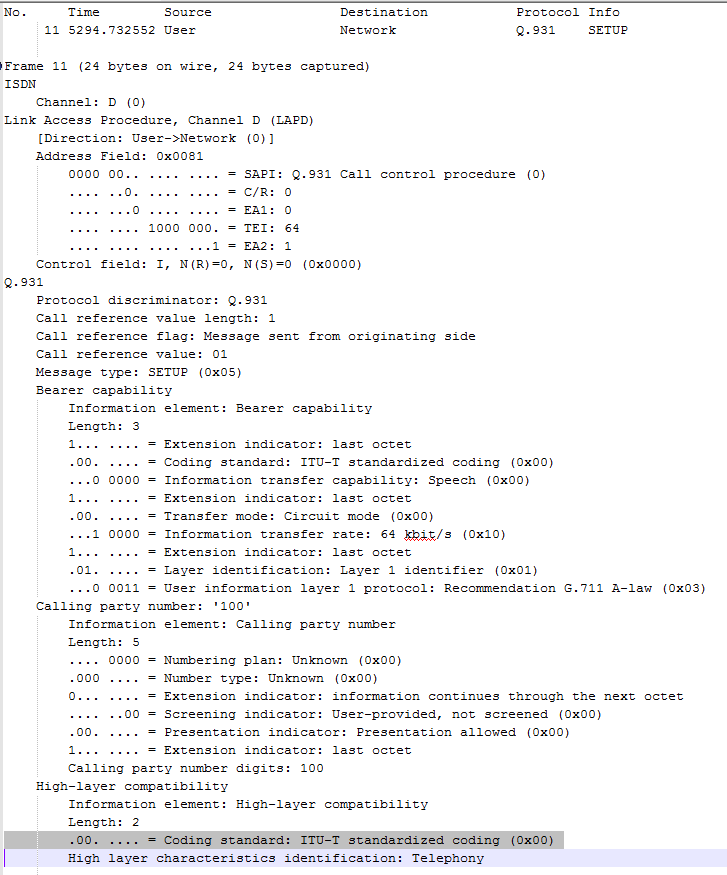
\includegraphics[width=0.8\textwidth]{tkinhalt/ba_bilder/ba/itu_code.png}
		\caption{Verwendete Codecs}
		\label{codecs} 
		\end{figure}
		
	\item \textbf{Welche MSN-Nummer wird in welchem Rahmen �bertragen?}\newline
	Im Setup Frame, welches man in der vorherigen Frage bereits betrachten konnte, wird die MSN des anrufenden Teilnehmers �bertragen. Zu finden ist diese unter dem Abschnitt Q.931 als Callin Party-Number. Die MSN des Teilnehmers auf der anderen Seite steht die MSN in dem Connect Rahmen. Diese ist ebenfalls im Abschnitt Q.931 unter Connected Number zu sehen.
		\begin{figure}[H]
		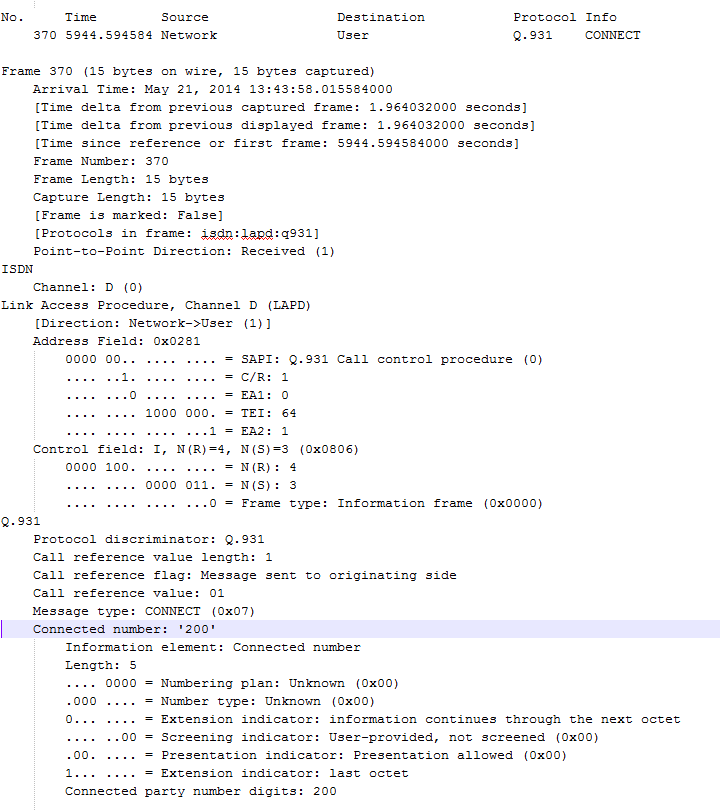
\includegraphics[width=0.8\textwidth]{tkinhalt/ba_bilder/ba/connect_a5.png} 
		\caption{Connect Nachricht}
		\label{connect_nachricht}
		\end{figure}
		
	\item \textbf{Wann ist der gesicherte Aufbau der Schicht 3 abgeschlossen?}\newline
	Die Schicht 3 ist aufgebaut, sobald das Netzwerk dem User eine Seup-Acknoledgment-Nachricht �bersendet. Diese best�tigt die vom User gesendete Setup-Nachricht und dass alles gut gegangen ist. 
	\begin{figure}[H]
	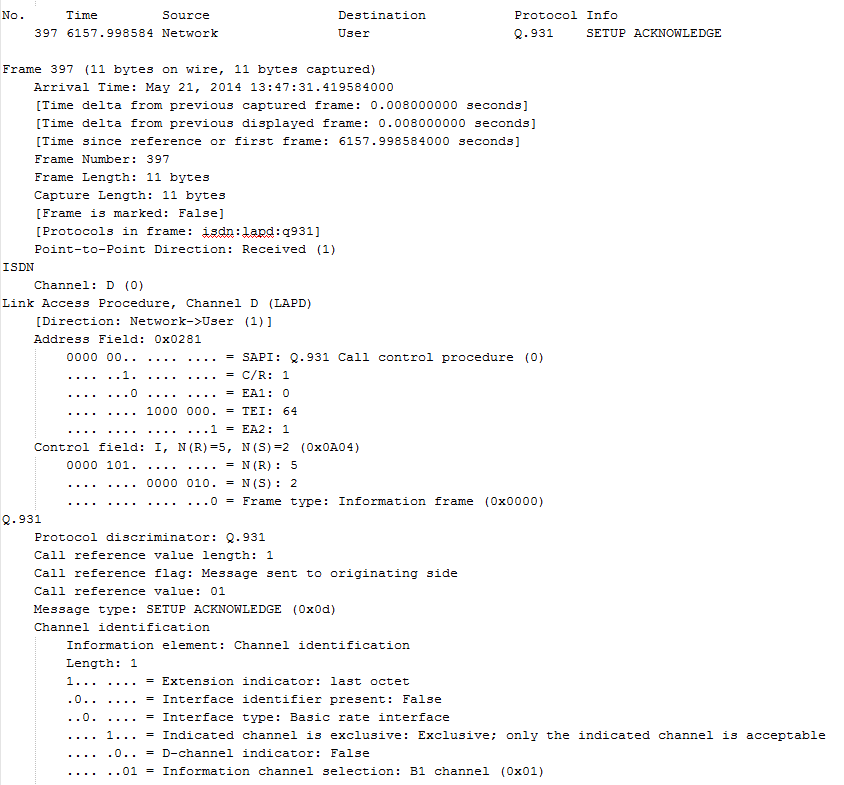
\includegraphics[width=0.8\textwidth]{tkinhalt/ba_bilder/ba/setup_acknoledge_a6.png}
	\caption{Setup Acknowledge}
	\label{setup_acknowledge}
	\end{figure}

	\item \textbf{Welchen B-Kanal weist die Vermittlung der Verbindung zu?}\newline
	In dem Call Proceeding-Frame findet man die Angabe zu dem genutzten Channel. In unserem Fall w�re das unter Q.931, 
	Information channel selection: B1 channel (0x01. Dies gibt an das der genutzte Channel hier der B1 ist. 
	\begin{figure}[H]
	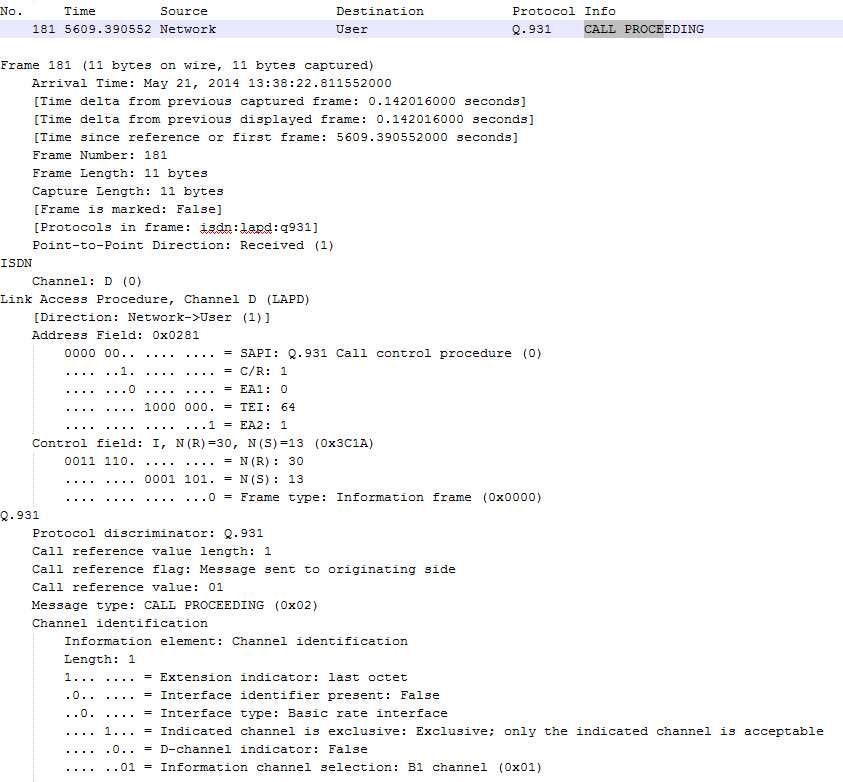
\includegraphics[width=0.8\textwidth]{tkinhalt/ba_bilder/ba/call-proceeding_a7.png}
	\caption{Call Proceeding Nachricht}
	\label{call_proceeding_nachricht}
	\end{figure}

	\item \textbf{Wo wird die gerufene Telefonnummer �bermittelt?}\newline
	Die Information-Frames senden bereits Teile der Rufnummer bevor die eigentliche Vermittlung anf�ngt. In unserem Fall werden hier insgesamt 		drei Frames gesendet die jeweils einer Nummer enthalten. Aufgrund der �bersichtlichkeit sind die Frames stark gek�rzt und direkt 				hintereinander gesetzt. 
	
	\begin{figure}[H]
	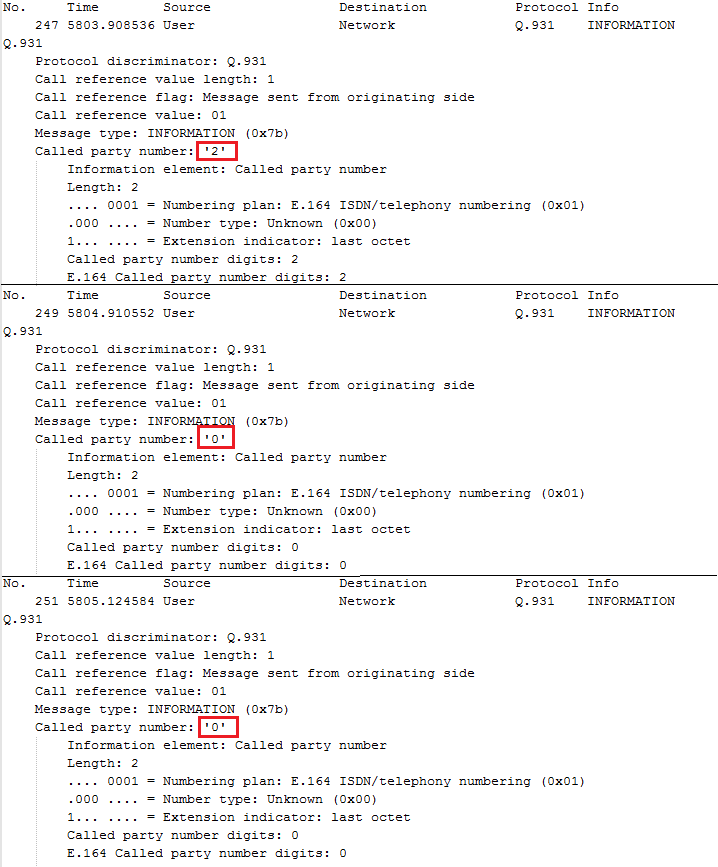
\includegraphics[width=0.8\textwidth]{tkinhalt/ba_bilder/ba/information_a8.png}
	\caption{Informations Rahmen}
	\label{info_rahmen}
	\end{figure}

	\item \textbf{Mit welchem Rahmen best�tigt die Vermittlung die Vollst�ndigkeit der Rufnummer und beginnt den angeforderten Teilnehmer anzuw�hlen?}\newline
	Nachdem alle Ziffern gesendet worden sind und die Vermittlungstelle diese als g�ltige Rufnummer erkannt hat sendet sie einen Call Proceeding-Frame an das Telefon und es wird keine weitere Ziffer mehr angenommen. Nun beginnt die Anwahl des anderen Teilnehmers. Der Call-Proceeding-Frame ist bereits zwei Fragen vorher gezeigt worden und wird deshalb hier nicht noch einmal aufgef�hrt.

	\item \textbf{Mit welchem Rahmen signalisiert die Vermittlung, dass der gerufene Teilnehmeranschluss ein Endger�t besitzt, das den Sprachdienst erf�llen kann und ein Rufsignal aussendet?}
	
	
	Jedes Endger�t das den Anruf annehmen kann sendet eine Alerting Nachricht und beginnt darauf hin zu Klingeln.
	
	\begin{figure}[H]
	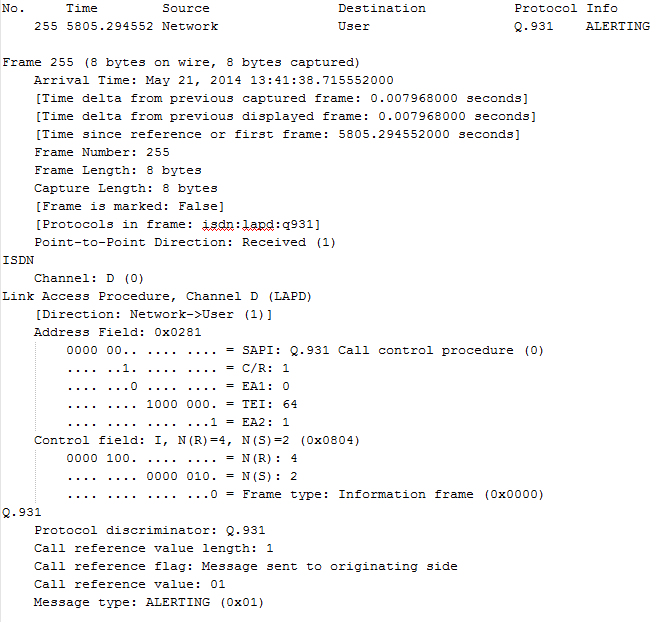
\includegraphics[width=0.8\textwidth]{tkinhalt/ba_bilder/ba/alerting_a9.png}
	\caption{Alert Frame}
	\label{alert_frame}
	\end{figure}

	\item \textbf{Wann sind die Schichten 3 und 2 jeweils wieder vollst�ndig abgebaut?}\newline
	Nachdem das Netzwerk eine Realease Complete Nachricht gesendet hat sind alle vorher belegten Kan�le wieder frei und Schicht 3, sowie Schicht 2 wieder abgebaut.
	
	\begin{figure}[H]
	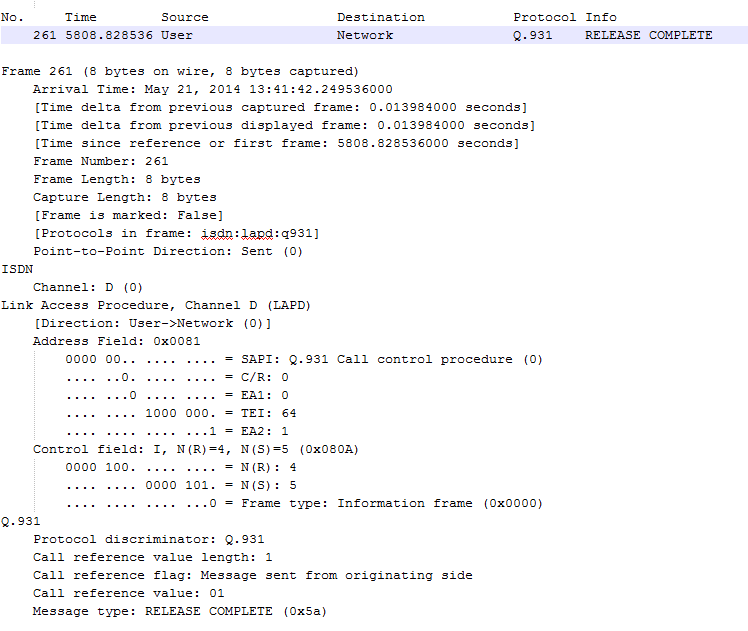
\includegraphics[width=0.8\textwidth]{tkinhalt/ba_bilder/ba/Release-Complete.png}
	\caption{Realease Complete Frame}
	\label{release_complete}
	\end{figure}
	

	\item \textbf{Bei ISDN gibt es die M�glichkeit, bei einem abgehenden Ruf die Zielrufnummer vor oder nach dem Abheben des H�rers einzugeben. Wodurch unterscheidet sich die Signalisierung auf Schicht 3 (SETUP- und INFO Nachricht) der Teilnehmerschnittstelle in diesen beiden F�llen?}\newline
Durch Abnehmen des H�rers wird f�r gew�hnlich eine Setup Nachricht gesendet wodurch bereits eine Verbindung zur Vermittlungsstelle aufgebaut wird. Nimmt der Teilnehmer also erst den H�rer ab k�nnen bereits die ersten Ziffern �berliefert werden. Dieser Vorgang ist durch den Versuch gut nachvollziehbar. Im Gegensatz dazu kann der Nutzer ebenfalls die Ziffern erst tippen und dann den H�rer abnehmen. Dies hat zur Folge, dass die ben�tigten Ziffern bereits vorhanden sind bevor die Setup-Nachricht gesendet wird. Dadurch k�nnen die Ziffern direkt in der Setup-Nachricht mit gesendet werden. Der folgende Frame zeigt das bereits die Called-Party-Number eingetragen ist. Hier wird das Endger�t mit der Nummer 100 von dem Endger�t mir der Nummer 200 angerufen. Der Frame wurde aufgrund der Gr��e etwas zugeschnitten, er enth�lt jedoch alle wichtigen Informationen.
	
	\begin{figure}[H]
	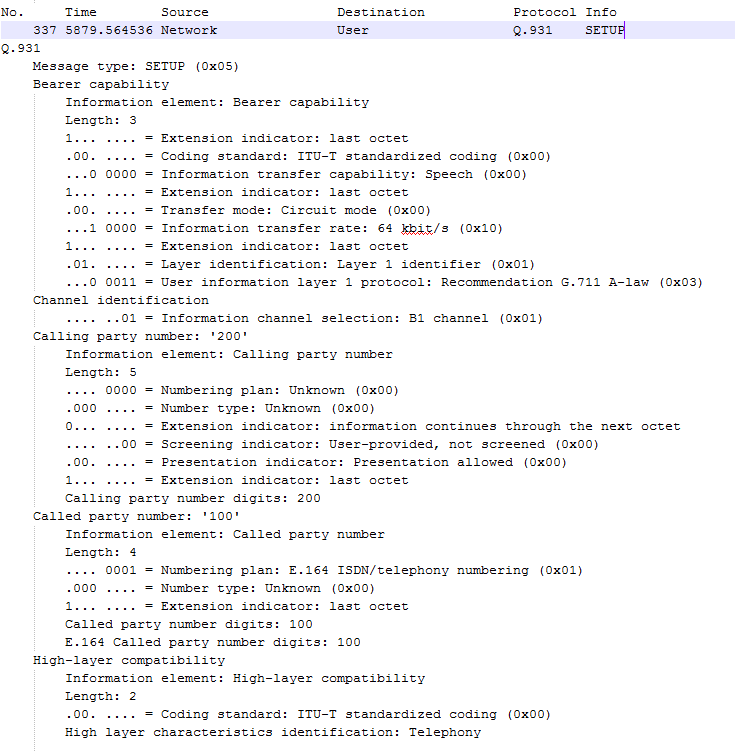
\includegraphics[width=0.8\textwidth]{tkinhalt/ba_bilder/ba/letzte_setup_block.png}
	\caption{Setup Nachricht mit vollst�ndiger Rufnummer}
	\label{setup_block_nachricht}
	\end{figure}
	
\end{enumerate}

%\begin{table}
%\begin{tabular}{|p{0.20 \linewidth}||*{9}{p{0.07 \linewidth}|}}
%\hline
%\diagbox{Nachricht} { Nachrichtenelement} & Alert & Call Proc & Conn & DISC & Info & Rel & Rel. Comp & Setup & Setup Ack\\
%\hline
%\hline
%Bearer Capability &  & & & & & & & &    \\ 
%\hline
%Cause & & & & & & & & &  \\
%\hline
%Channel Identification  & & & & & & & & &  \\
%\hline
%Process Indicator  & & & & & & & & &  \\
%\hline
%Display  & & & & & & & & &  \\
%\hline
%Date / Time  & & & & & & & & &  \\
%\hline
%Calling Party Number  & & & & & & & & & \\
%\hline
%Called Party Number   & & & & & & & & & \\
%\hline
%Sending Complete  & & & & & & & & & \\
%\hline
%Facility  & & & & & & & & & \\
%\hline
%User to User Information  & & & & & & & & & \\
%\hline
%\end{tabular}
%\caption{Genutzte Nachrichten}
%\end{table}
 		% Abschlussarbeit geht!
%=========================================
% 	   Einleitung     		 =
%=========================================

\chapter{RSP Versuch \label{rspVersuch}}
\section{Einleitung}
Router und Switche begleiten uns im t�glichen Leben. Auch wenn sie oft nicht wahrgenommen werden, sind sie doch allgegenw�rtig. Ob mobiles Surfen, das Surfen am Computer oder auch telefonieren, diese T�tigkeiten sind ohne Router und Switche nicht m�glich. Der Netzwerkausr�ster Cisco Systems rechnet bis zum Jahr 2018 mit einem weltweiten Internettraffic von 1,6 Zettabyte \cite{cisco_traffic_schaetzung}. Die Netzwerke, die diesen Traffic behandeln und abwickeln sollen wachsen stetig mit ihren Aufgaben. Deswegen ist eine fundierte Ausbildung in der Netzwerktechnik und ein Verst�ndnis der Komponenten f�r den Informatiker der Zukunft unausweichlich. 
Der folgende Versuch soll einen grundlegenden Einblick in den Aufbau eines Netzwerkes und die Konfiguration der Komponenten vermitteln.

\subsection{Ben�tigte Hardware f�r den Versuch}
F�r den Versuch werden ein Cisco 2811 Router und ein Cisco 2960 Switch ben�tigt. Zus�tzlich werden ein Windows Computer mit einem Terminal Emulationsprogramm und diverse Kabel ben�tigt.

\subsubsection{Router}
Die Aufgabe eines Routers, manchmal auch als Layer 3 Switch bezeichnet, ist es, zwischen mehreren Netzwerken der ISO/OSI Referenzmodell Schicht 3 zu vermitteln. Dazu besitzt ein Router mehrere (virtuelle) Ports, an denen die entsprechenden Netzwerke angeschlossen sind. Der Router, der f�r unseren Versuch zur Verf�gung stand ist vom Netzwerkausr�ster Cisco Systems und ist aus der Modellreihe 2811.

\begin{figure}[htbp] 
  \centering
     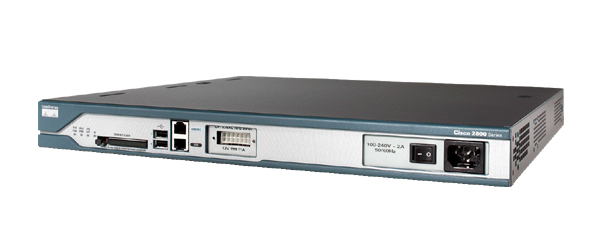
\includegraphics[width=0.6\textwidth]{tkinhalt/rsp_bilder/router.jpg}
  \caption{Ein Cisco 2800 Router \cite{cisco_2800_router}}
  \label{fig:router}
\end{figure}

\subsubsection{Switch}
Die Aufgabe eines Switches ist es, Netzwerksegmente miteinander zu verbinden. Das bedeutet, dass mehrere Kabel physikalisch miteinander verbunden werden k�nnen und die Datenpakete von einem Kabel in ein anderes weitergeleitet werden k�nnen. Logisch gesehen, werden die Datenpakete nur an die Kabel oder Ports weitergeleitet, die die Empf�ngeradresse dieses Pakets haben. Im Versuch stand uns ein Switch aus der Serie 2960 vom Netzwerkausr�ster Cisco Systems zur Verf�gung.

 \begin{figure}[htbp] 
  \centering
     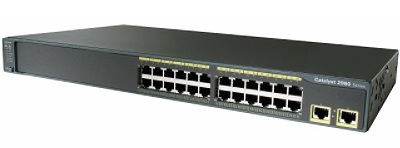
\includegraphics[width=0.6\textwidth]{tkinhalt/rsp_bilder/switch.jpg}
  \caption{Ein Cisco 2960 Switch \cite{cisco_2960_switch}}
  \label{fig:switch}
\end{figure}

\subsubsection{Kabel \label{kabel}}
Bei den Kabeln gibt es verschiedene Typen. Bei den Kabeln zur Energieversorgung der Ger�te handelt es sich um normale Kaltger�tekabel, diese brauchen an dieser Stelle nicht weiter beschrieben zu werden. Weiterhin waren RJ 45 Twisted Pair Kabel verwendet. Diese dienen der Verbindung zwischen den Routen, bzw. zwischen Switchen und Computern. %\todo{War da auch ein Crossover Kabel dabei?} 
Diese Verbindung dient dem Austausch von Nutzdaten. Die Konfiguration wurde �ber eine serielle Schnittstelle vorgenommen. Das dazugeh�rige Kabel hat auf der einen Seite einen female COM Port, auf der anderen Seite einen male RJ 45 Stecker. 

\subsubsection{Hintergrund der seriellen �bertragung}
Im Abschnitt \ref{kabel} wurde erw�hnt, dass f�r die Konfiguration die serielle Schnittstelle genutzt wird. Dabei stellt sich die Frage, warum dieser Aufwand betrieben werden muss, obwohl ein Switch doch mit ausreichend Ethernet Ports ausgestattet sein sollte. Den Hintergrund m�chten wir an dieser Stelle durch ein Beispiel beleuchten:
\begin{enumerate}
	\item Router und Computer befinden sich im Netzwerk 192.168.0.0/16
	\item Der Administrator will das Netzwerk in das Netzwerk 172.16.0.0/12 umbenennen
	\item Der Administrator vertippt sich bei der Vergabe der Ip und gibt die Netzwerkadresse 172.36.0.0 ein
\end{enumerate}

Was wird nun passieren? Wir setzen voraus, dass im Netzwerk kein DHCP Server aktiviert ist und alle Ip Adressen statisch vergeben werden. Im ersten Schritt ist die Welt noch in Ordnung. Im zweiten Schritt �ndert der Administrator die NW Adressen seines Computers und die des Routers. Im dritten Schritt bricht das Chaos aus. Mit dem Abspeichern der ersten Adresse, sei es Computer oder Router, verliert der Administrator die Kontrolle �ber den Router. Da sich mit einer ge�nderten Adresse der Router und der Computer in verschieden Netzwerken befinden, ist dieser \glqq Fehler\grqq~ vorhersehbar und leicht nachzuvollziehen. Der Administrator ber�cksichtigt diese Tatsache und speichert zuerst die Konfiguration des Routers. Nachdem er die Verbindung zum Router verloren hat speichert er die neue Konfiguration im Computer. Obwohl sich Computer und Router vermeintlich wieder in den gleichen Netzen befinden, hat er keinen Zugriff mehr auf den Router.

Ohne einen logischen Zugriff auf den Router gestaltet sich die Suche nach dem Fehler sehr schwierig. Diese Problematik kann durch die Konfiguration �ber die serielle Schnittstelle vermieden werden. Ein weiterer Vorteil ist,  dass die Konfigurationsschnittstelle des Switches vom Rest des Netzwerkes getrennt ist. Dadurch kann alleine schon durch die Trennung ein Angriff auf den Switch erschwert werden.
\section{Der Umgang mit Physikalischen Ger�ten}
Die physische Einrichtung des Systems ist in der Aufgabenstellung genau beschrieben. So viel sei zu sagen, jeder der beiden Computer ist per LAN Schnittstelle mit dem Switch verbunden. Je ein Computer ist �ber den COM Port (seriell) mit Router und Switch verbunden. Router und Switch sind �ber Gigabit Ethernet miteinander verbunden.

Die logische Einrichtung des Systems geschieht �ber Hyper Terminal. Hyperterminal ist eine Terminal Emulationssoftware. Diese erm�glicht eine Verbindung zu anderen Computern oder Gro�rechnern �ber die serielle Schnittstelle. Diese Verbindung ist rein ASCII textbasiert. 

\subsection{Einrichtung eines Switchs}
Die Einrichtung des Switches beginnt mit dem Hochfahren des Ger�ts. Dabei kann im Hyperterminal �berwacht werden, ob der Switch ordnungsgem�� startet. Nachdem die Selbstdiagnose durchgelaufen ist, kann in den Auf�hrungsmodus, bzw. in den \glqq  privileged EXEC mode\grqq ~gewechselt werden.

Die unterschiedlichen Kommando Modi sind in Tabelle \ref{ciscoCommandMode} aufgef�hrt.  

\begin{table}
\begin{tabular}{|p{0.15 \linewidth} | p{0.3 \linewidth} | p{.15\linewidth} | p{0.3 \linewidth} |}
\hline
Command Mode  & Access Method & Prompt & Exit \\
\hline
\hline
User EXEC & This is the first level of access. Change terminal settings, perform basic tasks, and list system information. & \textit{ap>} & Enter the logout command.    \\ 
\hline
Privileged EXEC & From user EXEC mode, enter the enable command. & \textit{ap\#} & To exit to user EXEC mode, enter the disable command. \\
\hline
Global configuration  & From privileged EXEC mode, enter the configure command. & \textit{ap(config)\#} & To exit to privileged EXEC mode, enter the exit or end command, or press Ctrl-Z.  \\
\hline
Interface configuration  & From global configuration mode, specify terminal then specify an interface by entering the interface command followed by the interface type and number. & \textit{ap(config-if)\#} & To exit to privileged EXEC mode, enter the end command, or press Ctrl-Z. To exit to global configuration mode, enter the exit command.  \\
\hline
\end{tabular}
\caption{Die unterschiedlichen Command Modi von IOS}
\label{ciscoCommandMode}
\end{table}

Im privileged EXEC mode m�ssen erst die Einstellungen des Switches zur�ckgesetzt werden. Dadurch wird vermieden, dass bereits bestehende Konfigurationen die Ergebnisse beeinflussen. Die Ausgabe ist �hnlich der Ausgabe \ref{routerZurueckSetzen}. Durch die Befehle \textit{delete flash : vlan.dat} und \textit{erase startup-config} werden erst die Einstellungen zu den V-Lan gel�scht und anschlie�end wird die gesamte Konfiguration gel�scht. 

\fbox{\parbox{\textwidth}{
	\textbf{Der Unterschied zwischen \textit{erase startup-config} und \textit{erase running-config}:} Auf den ersten Blick haben beide Befehle die gleiche Wirkung. Der Unterschied ist, dass die Konfiguration nach einem Neustart des Ger�ts wieder hergestellt wird, wenn  \textit{erase running-config} genutzt wurde. Wurde \textit{erase startup-config} genutzt, ist die Konfiguration dauerhaft gel�scht. Der genaue Unterschied wird nach dem Lesen der Erkl�rung von Speicherunterschieden \ref{aufzaehlungSpeichertypen} deutlicher.
}}

Nachdem die Konfiguration des Switches zur�ckgesetzt wurde, kommt die Aufforderung, den Switch zu konfigurieren. Diese Aufforderung wird mit einem \textit{n} quittiert. Dadurch wird die Konfiguration nicht durchgef�hrt und der Switch l�uft mit seinen Default Konfigurationen. Der Switch ist jetzt bereit f�r den weiteren Versuch.


\subsection{Konfiguration eines Routers}
Das Zur�cksetzen des Routers geschieht analog zu dem Zur�cksetzen des Switches. 

\begin{lstlisting}[captionpos=b, caption=Die Ausgabe des Zur�cksetzens, label=routerZurueckSetzen]
	Router#erase startup-config
Erasing the nvram filesystem will remove all configuration files! Continue? [confirm]
[OK]
Erase of nvram: complete
Router#
*Jun  4 10:44:29.415: %SYS-7-NV_BLOCK_INIT: Initialized the geometry of nvram
Router#re
*Jun  4 10:45:30.887: %LINK-3-UPDOWN: Interface Serial0/0/0, changed state to do
wn
*Jun  4 10:45:31.887: %LINEPROTO-5-UPDOWN: Line protocol on Interface Serial0/0/
0, changed state to do
Router#reload
Proceed with reload? [confirm]

*Jun  4 10:45:44.707: %SYS-5-RELOAD: Reload requested  by console. Reload Reason
: Reload Command.

System Bootstrap, Version 12.4(13r)T11, RELEASE SOFTWARE (fc1)
Technical Support: http://www.cisco.com/techsupport
Copyright (c) 2009 by cisco Systems, Inc.

Initializing memory for ECC
.
c2811 platform with 262144 Kbytes of main memory
Main memory is configured to 64 bit mode with ECC enabled


Upgrade ROMMON initialized
program load complete, entry point: 0x8000f000, size: 0xcb80
program load complete, entry point: 0x8000f000, size: 0xcb80

program load complete, entry point: 0x8000f000, size: 0x1859ee4
Self decompressing the image : #################################################
###########################################
#####################################
########### [OK]

Smart Init is enabled
smart init is sizing iomem
  ID            MEMORY_REQ                 TYPE
0003E7          0X00473800 C2811 Mainboard
                0X000021B8 Onboard USB
                0X002C29F0 public buffer pools
                0X00211000 public particle pools
TOTAL:          0X009493A8

If any of the above Memory Requirements are
"UNKNOWN", you may be using an unsupported
configuration or there is a software problem and
system operation may be compromised.
Rounded IOMEM up to: 10Mb.
Using 3 percent iomem. [10Mb/256Mb]

[...]

Cisco 2811 (revision 49.46) with 251904K/10240K bytes of memory.
Processor board ID FCZ131871SX
2 FastEthernet interfaces
2 Low-speed serial(sync/async) interfaces
DRAM configuration is 64 bits wide with parity enabled.
239K bytes of non-volatile configuration memory.
62720K bytes of ATA CompactFlash (Read/Write)


         --- System Configuration Dialog ---
         
\end{lstlisting}

Nachdem der Router auf die Grundeinstellungen zur�ck gesetzt wurde, muss er neu konfiguriert werden. Der folgende Dialog startet die Konfiguration: 

\begin{lstlisting}[captionpos=b, caption=Die Aufforderung zum neukonfigurieren des Routers, label=routerNeuKonfigurieren]
Would you like to enter the initial configuration dialog? [yes/no]: yes

At any point you may enter a question mark '?' for help.
Use ctrl-c to abort configuration dialog at any prompt.
Default settings are in square brackets '[]'.

Basic management setup configures only enough connectivity
for management of the system, extended setup will ask you
to configure each interface on the system

Would you like to enter basic management setup? [yes/no]: yes
Configuring global parameters:
\end{lstlisting}

Im Gegensatz zum Switch wird der Router konfiguriert. Dies geschieht �ber den Befehl \textit{yes}, oder einfach \textit{y}. Die Konfiguration wird nach den Vorgaben der Versuchsbeschreibung durchgef�hrt. Sowohl vor, als auch nach dem Konfigurieren wird das Kommando \textit{show running-config} aufgerufen. 
\begin{lstlisting}[captionpos=b, caption=Die Ausgabe der Konfiguration vor dem Konfigurieren, label=konfigVor]
Password:
Router#enable
Router#show running-config
Building configuration...

Current configuration : 1058 bytes
!
version 12.4
service timestamps debug datetime msec
service timestamps log datetime msec
no service password-encryption
!
hostname Router
!
boot-start-marker
boot-end-marker
!
enable secret 5 $1$WPnk$wNZGar7F/KHiw5VcuCMtE.
enable password cisco
!
no aaa new-model
!
!
ip cef
!
!
no ip domain lookup
multilink bundle-name authenticated
!
!
!
archive
 log config
  hidekeys
!
!
!
!
!
interface FastEthernet0/0
 description R1 LAN Default Gateway
 ip address 192.168.1.1 255.255.255.128
 duplex auto
 speed auto
!
interface FastEthernet0/1
 no ip address
 shutdown
 duplex auto
 speed auto
!
interface Serial0/0/0
 description R1 WAN
 ip address 192.168.1.193 255.255.255.252
 clock rate 125000
!
interface Serial0/0/1
 no ip address
 shutdown
 clock rate 125000
!
router rip
 version 2
 network 192.168.1.0
!
ip forward-protocol nd
!
!
ip http server
!
!
!
control-plane
!
banner motd ^CUnauthorized Use Prohibited^C
!
line con 0
 password cisco
 logging synchronous
 login
line aux 0
line vty 0 4
 password cisco
 login
!
scheduler allocate 20000 1000
!
end
\end{lstlisting}

Nach dem Konfigurieren sieht die Ausgabe folgenderma�en aus:
\begin{lstlisting}[captionpos=b, caption=Die Ausgabe der Konfiguration nach dem Konfigurieren, label=configRouterKonfiguriert]
R1_HTW#show running-config
Building configuration...

Current configuration : 1058 bytes
!
version 12.4
service timestamps debug datetime msec
service timestamps log datetime msec
no service password-encryption
!
hostname R1_HTW
!
boot-start-marker
boot-end-marker
!
enable secret 5 $1$WPnk$wNZGar7F/KHiw5VcuCMtE.
enable password cisco
!
no aaa new-model
!
!
ip cef
!
!
no ip domain lookup
multilink bundle-name authenticated
!
!
!
archive
 log config
  hidekeys
!
!
!
!
!
interface FastEthernet0/0
 description R1 LAN Default Gateway
 ip address 192.168.1.1 255.255.255.128
 duplex auto
 speed auto
!
interface FastEthernet0/1
 no ip address
 shutdown
 duplex auto
 speed auto
!
interface Serial0/0/0
 description R1 WAN
 ip address 192.168.1.193 255.255.255.252
 clock rate 125000
!
interface Serial0/0/1
 no ip address
 shutdown
 clock rate 125000
!
router rip
 version 2
 network 192.168.1.0
!
ip forward-protocol nd
!
!
ip http server
!
!
!
control-plane
!
banner motd ^CUnauthorized Use Prohibited^C
!
line con 0
 password cisco
 logging synchronous
 login
line aux 0
line vty 0 4
 password cisco
 login
!
scheduler allocate 20000 1000
!
end
\end{lstlisting}

Zwischen den beiden Ausgaben gibt es augenscheinliche Merkmale:

Der Unterschied zeigt sich im Hostname. Dieser Unterschied deckt sich mit den Erwartungen, da bis auf den Hostname nichts konfiguriert wurde.

\begin{lstlisting}[captionpos=b, caption=Die Ausgabe der Startup Config]
R1_HTW#show startup-config
Using 1039 out of 245752 bytes
!
version 12.4
service timestamps debug datetime msec
service timestamps log datetime msec
no service password-encryption
!
hostname Router
!
boot-start-marker
boot-end-marker
!
enable secret 5 $1$WPnk$wNZGar7F/KHiw5VcuCMtE.
enable password cisco
!
no aaa new-model
!
!
ip cef
!
!
no ip domain lookup
multilink bundle-name authenticated
!
!
!
archive
 log config
  hidekeys
!
!
!
!
!
interface FastEthernet0/0
 description R1 LAN Default Gateway
 ip address 192.168.1.1 255.255.255.128
 duplex auto
 speed auto
!
interface FastEthernet0/1
 no ip address
 shutdown
 duplex auto
 speed auto
!
interface Serial0/0/0
 description R1 WAN
 ip address 192.168.1.193 255.255.255.252
!
interface Serial0/0/1
 no ip address
 shutdown
 clock rate 125000
!
router rip
 version 2
 network 192.168.1.0
!
ip forward-protocol nd
!
!
ip http server
!
!
!
control-plane
!
banner motd ^CUnauthorized Use Prohibited^C
!
line con 0
 password cisco
 logging synchronous
 login
line aux 0
line vty 0 4
 password cisco
 login
!
scheduler allocate 20000 1000
!
end
\end{lstlisting}

Ein Unterschied zwischen \textit{show running-config} und \textit{show startup-config} ist der Unterschied der Hostnamen. Der Unterschied zwischen der running config und der startup config besteht darin, dass die startup config im NVRAM des Routers gespeichert ist, die running config ist im RAM gespeichert. Da die �nderungen sich nur auf den fl�chtigen Speicher beschr�nken, gehen sie bei einem Neustart des Routers verloren.

Um die Auswirkungen des n�chsten Schritts zu verstehen, ist es sinnvoll sich die verschiedenen Sorten von Speicher in einem Cisco Router vor Augen zu f�hren. Die Erl�uterungen zu den Speichersorten stammen von Cisco \cite{speicherTypen}

\label{aufzaehlungSpeichertypen}
\begin{itemize}
	\item \textbf{RAM: }Random Access Memory ist der fl�chtige Arbeitsspeicher, von Cisco auch als Dynamic RAM bezeichnet. Fl�chtig bedeutet, dass die gespeicherten Informationen nach einem Spannungsverlust verloren gehen. Im RAM werden ARP Tabellen, Routing Tabellen, eine tempor�re Konfiguration, Packet Queues, usw. gespeichert. Vor allem wird aber im RAM auch das entpackte Betriebssystem der Ger�te vorgehalten. Der Vorteil von RAM ist, dass er sehr schnell ist und f�r viele Schreib- und Lesevorg�nge ausgelegt ist.
	\item \textbf{Flash: } Der Flash Speicher beinhaltet bei Cisco Produkten ein Image oder mehrere Images des Betriebssystems. Der Flash Speicher beispielsweise genutzt, wenn das Betriebssystem des Routers neu aufgesetzt werden muss. Dies geschieht aus dem komprimierten Image vom Flash. Aber auch beim Starten des Switches wird ein Image vom Flash Speicher in den RAM geladen.
	\item \textbf{NVRAM: } Im NVRAM sind die Boot Konfigurationen gespeichert. Der Inhalt des NVRAMs geht nicht verloren, wenn der Router neu gestartet wird, oder durch einen Stromausfall unterversorgt wird. 
	\item \textbf{ROM: } Der ROM speichert beispielsweise Informationen, die f�r den Selbsttest des Routers n�tig sind. Da aus dem ROM nur gelesen werden kann, m�ssen f�r ein Software Update einige ROM Speichersteine ausgetauscht werden.
\end{itemize}

Die Konfiguration ist im aktuellen Stadium des Versuchs lediglich im RAM. Der Befehl \textit{copy running-config startup-config} kopiert die Konfiguration aus dem RAM in den NVRAM. 

\begin{lstlisting}
R1_HTW#copy running-config startup-config
Destination filename [startup-config]?
Building configuration...
[OK]
\end{lstlisting}

Betrachten wir nun die startup config, sollte die Ausgabe wie die Ausgabe \ref{configRouterKonfiguriert} aussehen. 

\begin{lstlisting}[caption=Die Startup Config nach dem Kopieren in den NVRAM]
R1_HTW#show startup-config
Using 1058 out of 245752 bytes
!
version 12.4
service timestamps debug datetime msec
service timestamps log datetime msec
no service password-encryption
!
hostname R1_HTW
!
boot-start-marker
boot-end-marker
!
enable secret 5 $1$WPnk$wNZGar7F/KHiw5VcuCMtE.
enable password cisco
!
no aaa new-model
!
!
ip cef
!
!
no ip domain lookup
multilink bundle-name authenticated
!
!
!
archive
 log config
  hidekeys
!
!
!
!
!
interface FastEthernet0/0
 description R1 LAN Default Gateway
 ip address 192.168.1.1 255.255.255.128
 duplex auto
 speed auto
!
interface FastEthernet0/1
 no ip address
 shutdown
 duplex auto
 speed auto
!
interface Serial0/0/0
 description R1 WAN
 ip address 192.168.1.193 255.255.255.252
 clock rate 125000
!
interface Serial0/0/1
 no ip address
 shutdown
 clock rate 125000
!
router rip
 version 2
 network 192.168.1.0
!
ip forward-protocol nd
!
!
ip http server
!
!
!
control-plane
!
banner motd ^CUnauthorized Use Prohibited^C
!
line con 0
 password cisco
 logging synchronous
 login
line aux 0
line vty 0 4
 password cisco
 login
!
scheduler allocate 20000 1000
!
end
\end{lstlisting}

Um zu testen, ob das Kopieren der Konfig Datei vom RAM in den NVRAM bietet sich ein Neustart des Routers an. Da der RAM fl�chtig ist, sollte ja die Konfiguration verworfen werden, wenn sie nur im RAM gespeichert ist. Den Router kann man mit dem Befehl \textit{reload} neu starten. Um die Aussage pr�ziser zu machen, der Befehl reload stoppt nur das System. Wenn es als \textit{restart on error} konfiguriert ist, bzw. nicht anders konfiguriert wurde, startet es automatisch neu.

Vor dem Test, ob die Konfiguration immer noch g�ltig ist, betrachten wir das Terminal beim Hochfahren des Routers.
\begin{lstlisting}
R1_HTW#reload
Proceed with reload? [confirm]

*May 28 11:12:44.035: %SYS-5-RELOAD: Reload requested  by console. Reload Reason
: Reload Command.

System Bootstrap, Version 12.4(13r)T11, RELEASE SOFTWARE (fc1)
Technical Support: http://www.cisco.com/techsupport
Copyright (c) 2009 by cisco Systems, Inc.

Initializing memory for ECC
.
c2811 platform with 262144 Kbytes of main memory
Main memory is configured to 64 bit mode with ECC enabled


Upgrade ROMMON initialized
program load complete, entry point: 0x8000f000, size: 0xcb80
program load complete, entry point: 0x8000f000, size: 0xcb80

program load complete, entry point: 0x8000f000, size: 0x1859ee4
Self decompressing the image : ######################
###########################
##############################
##################################################
########### [OK]

Smart Init is enabled
smart init is sizing iomem
  ID            MEMORY_REQ                 TYPE
0003E7          0X00473800 C2811 Mainboard
                0X000021B8 Onboard USB
                0X002C29F0 public buffer pools
                0X00211000 public particle pools
TOTAL:          0X009493A8

If any of the above Memory Requirements are
"UNKNOWN", you may be using an unsupported
configuration or there is a software problem and
system operation may be compromised.
Rounded IOMEM up to: 10Mb.
Using 3 percent iomem. [10Mb/256Mb]

[...]



Press RETURN to get started!


*May 28 11:13:53.831: %LINK-3-UPDOWN: Interface FastEthernet0/0, changed state t
o up
*May 28 11:13:53.835: %LINK-3-UPDOWN: Interface FastEthernet0/1, changed state t
o up
*May 28 11:13:53.835: %LINK-3-UPDOWN: Interface Serial0/0/0, changed state to do
wn
*May 28 11:13:53.835: %LINK-3-UPDOWN: Interface Serial0/0/1, changed state to do
wn
*May 28 11:13:54.831: %LINEPROTO-5-UPDOWN: Line protocol on Interface FastEthern
et0/0, changed state to down
*May 28 11:13:54.835: %LINEPROTO-5-UPDOWN: Line protocol on Interface FastEthern
et0/1, changed state to down
*May 28 11:13:54.835: %LINEPROTO-5-UPDOWN: Line protocol on Interface Serial0/0/
0, changed state to down
*May 28 11:13:54.835: %LINEPROTO-5-UPDOWN: Line protocol on Interface Serial0/0/
1, changed state to down
*May 28 11:13:56.055: %SYS-5-CONFIG_I: Configured from memory by console
*May 28 11:13:56.455: %SYS-5-RESTART: System restarted --
Cisco IOS Software, 2800 Software (C2800NM-IPBASE-M), Version 12.4(15)T7, RELEAS
E SOFTWARE (fc3)
Technical Support: http://www.cisco.com/techsupport
Copyright (c) 1986-2008 by Cisco Systems, Inc.
Compiled Wed 13-Aug-08 17:09 by prod_rel_team
*May 28 11:13:56.463: %SNMP-5-COLDSTART: SNMP agent on host R1_HTW is undergoing
 a cold start
*May 28 11:13:56.759: %SYS-6-BOOTTIME: Time taken to reboot after reload =   73
seconds
*May 28 11:13:57.875: %LINK-5-CHANGED: Interface FastEthernet0/1, changed state
to administratively down
*May 28 11:13:57.939: %LINK-5-CHANGED: Interface Serial0/0/1, changed state to a
dministratively down
\end{lstlisting}

\subsection{Fazit des Versuchs}
Der Versuch hat uns die grunds�tzlich Einrichtung eines Cisco Routers n�her gebracht. Die grunds�tzliche Einrichtung umfasst sowohl die physikalische Verkabelung, als auch auch die Einrichtung der Software. 

Auf der physikalischen Seite haben wir die Interfaces von Routern und Switchen kennen gelernt. Die Interfaces k�nnen sowohl f�r den Payload sein, aber auch f�r die Konfiguration. Gerade bei der Konfiguration ist uns aufgefallen, dass sich hier die Profimodelle deutlich von den Ger�ten f�r den Heimbedarf unterscheiden. W�hrend die meisten Ger�te f�r den Heimbedarf weder separate Interfaces f�r Payload und Konfiguration, noch einen Unterschied zwischen einer fl�chtigen Konfiguration und einer dauerhaften Konfiguration haben, sind die Profiger�te doch bei der Konfiguration deutlich aufw�ndiger. Der h�here Aufwand erm�glich aber im Gegenzug eine deutlich feinere Konfiguration. 

Auf der logischen Seite haben wir etwas �ber die interne Arbeitsweise von Routern und Switchen gelernt. Diese Aussage bezieht sich auf die Berechtigungen und auf die verschiedenen Speicher innerhalb eines Ger�ts. Neben dieser Erkenntnis war der Versuch aber auch eine gelungene Einf�hrung in das Terminal von IOS. In diesem Zusammenhang ist mit IOS das Cisco Internetwork Operating System, also das Standard Betriebssystem von Cisco Routern und Switchen gemeint. Eine Verwechselung mit dem gleichnamigen Apple iOS, iPhone Operating System, soll hiermit ausgeschlossen werden.  

\section{Packet Tracer}
Packet Tracer ist eine Netzwerk Simulationssoftware der Firma Cisco Systems. Packet Tracer kann die Ger�te der Firma simulieren und erm�glicht so einen unkomplizierten Aufbau von Netzwerken. Der Vorteil von einer Simulationssoftware gegen�ber dem echten Aufbau ist, dass Fehler schnell korrigiert werden k�nnen und dass komplexe Zusammenh�nge anschaulich visualisiert werden k�nnen. 

F�r den Versuch ist nur ein Computer n�tig, der die entsprechende Software installiert hat.

Im folgenden wechseln die Namen der eingerichteten Computer. Dies ist der Versuchsbeschreibung geschuldet. An Passagen, an denen ein Wechsel des Namens die Ergebnisse des Versuchs unverst�ndlich machen kann, wird aufgrund der ge�nderten Namen genauer erkl�rt. %\todo{Oder habe ich mich irgendwo verhaspelt?}

\subsection{Aufbau des Netzwerkes}
\subsubsection{Ger�te}
Das virtuelle Netzwerk setzt sich aus zwei Computern, einem Switch und einem Router zusammen. Der Begriff \glqq virtuelles Netzwerk\grqq~steht in diesem Fall nicht mit dem Begriff \glqq v-Lan\grqq~im Zusammenhang, sondern soll ausdr�cken, dass dieses Netzwerk und die Ger�te von dem Programm simuliert werden. Der Aufbau wird in der Grafik \ref{fig:virtuellesNetzwerk} veranschaulicht.

 \begin{figure}[htbp] 
  \centering
     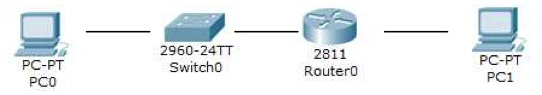
\includegraphics[width=0.8\textwidth]{tkinhalt/rsp_bilder/aufbauVirtuellesNetzwerk.jpg}
  \caption{Der Aufbau des virtuellen Netzwerks}
  \label{fig:virtuellesNetzwerk}
\end{figure}

\subsubsection{Adressvergabe}
Die in der Tabelle \ref{RSPadresstabelle} dargestellten Adressen stammen aus der Aufgabenbeschreibung des Versuchs. Interessant an diesem Aufbau ist, dass bis auf den Wechsel zwischen zwei v-Lan alle Standardsituationen in einem Netzwerk simuliert werden. 
 
\begin{table}
\begin{tabular}{|*{6}{c|}}
\hline
Device & Hostname & Interface & IP-Address & Subnet Mask & Default Gateway \\
\hline
\hline
PC0 & Labor-PC1 & Fast-Ethernet &  192.168.0.10 &  255.255.255.128 &  192.168.0.1 \\ 
\hline
Switch0 & Labor-Switch1 & FE0/1 u. FE0/2 & NA & NA & NA  \\
\hline
Router0 &  Labor-Router1 & FE0/0 &  192.168.0.1 & 255.255.255.128 & NA \\
\hline
 & &  FE0/1 & 10.10.10.1 &  255.255.255.224 & NA\\
\hline
PC1 & Labor-PC2 & Fast-Ethernet & 10.10.10.10 & 255.255.255.224 &  10.10.10.1 \\
\hline
\end{tabular}
\caption{Adresstabelle des Netzwerks}
\label{RSPadresstabelle}
\end{table}

\subsubsection{�berpr�fung des Testaufbaus}
Vertrauen ist gut, Kontrolle ist besser. Deswegen wird das soeben aufgebaute Netzwerk durch geeignete Pings getestet. Ping sendet lediglich ein ICMP echo request, wartet auf den echo reply und misst die ben�tigte Zeit. ICMP ist ein Bestandteil des Internet Protokolls, wird aber, je nach Literatur, als eigenst�ndiges Protokoll betrachtet. Es ist relativ zuverl�ssig und eine geeignete M�glichkeit zu testen, ob ein Host erreichbar ist. 


\begin{table}
\begin{tabular}{|*{5}{c|}}
\hline
\diagbox{Von}{Zu} & PC1 & PC2 & Router1 (FE0/0) & Router1 (FE0/1) \\
\hline
\hline
PC1 &   &  & 78ms & 62ms \\ 
\hline
PC2 & 82ms & &  &  35ms   \\
\hline
\end{tabular}
\caption{Ergebnisse des Ping}
\label{ergebnissePing}
\end{table}

Die Ergebnisse der Pings sind in der Tabelle \ref{ergebnissePing} zusammengefasst. Diese Ergebnisse sind bei n�herer Betrachtung interessant. Das Offensichtliche an den Ergebnissen ist, dass die Einrichtung des virtuellen Netzwerks scheinbar erfolgreich war. Betrachtet man die Zeiten genauer, f�llt auf, dass es in jeder Zeile eine kleinere Zeit und eine gr��ere Zeit gibt. In der Zeile PC2 f�llt dieser Unterschied besonders deutlich aus. 
Zu besseren �bersicht werden noch einmal die Hostnamen aufgel�st:

\textbf{10.10.10.10 $\rightarrow$ 192.168.0.10} = 82ms. Bei diesem Ping wurde das Netzwerk 10.10.10.0 verlassen und die Datenpakete mussten weiter geroutet werden. An diesem Prozess waren beide PC, der Router und der Switch beteiligt. Alleine aus der Anzahl der Ger�te ergibt sich eine Latenz, darauf addiert sich die Latenz des Routings.

\textbf{10.10.10.10 $\rightarrow$ 10.10.10.1} = 32ms. Dieser Ping hat das Netzwerk 10.10.10.0 nicht verlassen. Daher f�llt die Latenz des Routings weg. Auch, wenn durch die anderen Ger�te nur geringe Latenzen entstehen, PC1 und der Switch waren bei diesem Ping am Sendeprozess nicht beteiligt.

Die angegebenen Zeiten sind Mittelwerte, betrachtet man die Zeiten genauer, verst�rkt sich der Eindruck.
\begin{lstlisting}[captionpos=b, caption=Die genauen Zeiten ohne Routing , label=statisticsOhneRouting]
Ping statistics for 10.10.10.1:
    Packets: Sent = 4, Received = 4, Lost = 0 (0% loss),
Approximate round trip times in milli-seconds:
    Minimum = 17ms, Maximum = 62ms, Average = 35ms
\end{lstlisting}

\begin{lstlisting}[captionpos=b, caption=Die genauen Zeiten mit Routing , label=statisticsMitRouting]
Ping statistics for 192.168.0.10:
    Packets: Sent = 4, Received = 4, Lost = 0 (0% loss),
Approximate round trip times in milli-seconds:
    Minimum = 65ms, Maximum = 94ms, Average = 82ms
\end{lstlisting}

\subsection{Simulieren und Analysieren eines ECHO REQUEST/ECHO REPLY}
\subsubsection{Aufbau}
Der einzige Unterschied zum vorhergehenden Aufbau ist, dass die Software in den Simulationsmodus gewechselt wird. Dadurch ist es m�glich, die einzelnen Pakete grafisch darzustellen und ihren Weg durch das Netzwerk zu verfolgen. Zur Erinnerung, der Aufbau des virtuellen Netzwerks ist in der Grafik \ref{fig:virtuellesNetzwerk} dargestellt.

\subsubsection{Ablauf des Versuchs}
Von PC1 wird ein ein echo request zu PC2 gesendet. Dieser request soll von PC2 durch ein echo reply beantwortet werden. Dieser Weg entspricht einem Ping. Durch die Visualisierung von Packet Tracer kann anschaulich �berpr�ft werden, wie sich die Pakete und Frames bei den �berg�ngen zwischen den einzelnen Ger�ten verhalten.

\subsubsection{Auswertung des Versuchs}
 \begin{figure}[htbp] 
  \centering
     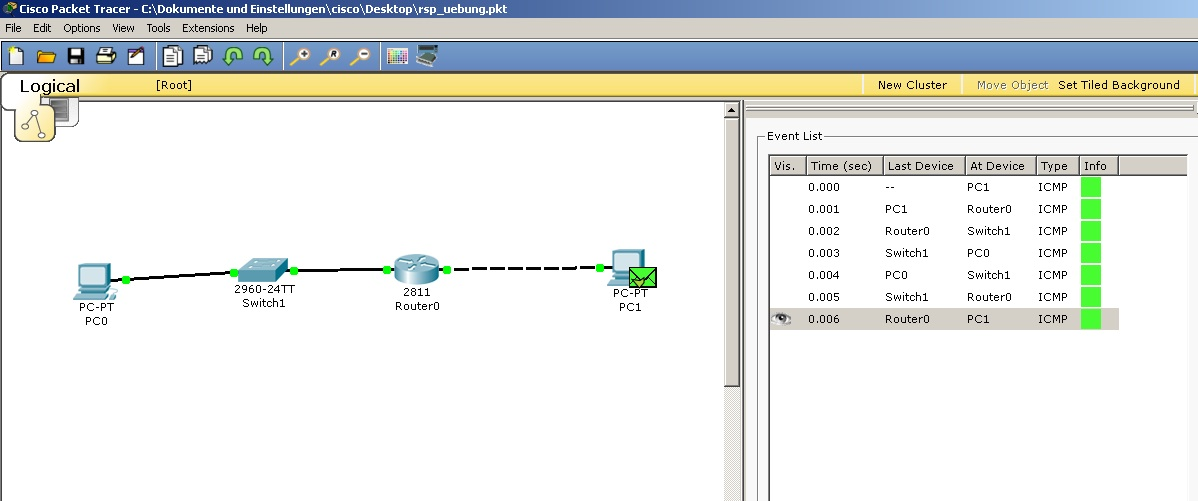
\includegraphics[width=0.8\textwidth]{tkinhalt/rsp_bilder/echoRequestStart.jpg}
  \caption{Der Beginn des echo request}
  \label{fig:startEchoRequest}
\end{figure}

Das Echo Paket befindet sich noch im PC1. Die Detailsicht ist in der Grafik \ref{fig:detailEchoRequestPC1} zu sehen. Dort sind sind die drei relevanten OSI Layer dargestellt. Im Layer 3 ist die IP Adresse von PC1 als Quelladresse und die IP Adresse von PC2 als Zieladresse zu sehen. Die Grafik \ref{fig:EchoRequestPC1} zeigt die gleiche ICMP Nachricht in der OSI Modell Darstellung. Da dort die relevanten Informationen zusammengefasst sind, werden wir uns im folgenden auf diese Ansicht beschr�nken. 

Die Ansicht, wie die ICMP Nachricht im Router aussieht ist in der Grafik \ref{fig:EchoRequestRouter}. Offensichtlich hat sich auf Layer 3 nichts ge�ndert. Das war auch zu erwarten, da es sich immer noch um den gleichen echo request handelt. Die Quelle ist weiterhin PC1 und das Ziel ist PC2. 

Eine Ver�nderung hat auf Layer 2 stattgefunden. Dort ist die Quelladresse die Zieladresse aus der Grafik \ref{fig:EchoRequestPC1}. Auch diese Beobachtung deckt sich mit den Erwartungen. Die ICMP Nachricht befindet sich im Layer 3. Da der Layer 3 auf die Sicherungsschicht, bzw. Layer 2, angewiesen ist, muss die ICMP Nachricht in ein Ethernet Frame verpackt werden. Der Router packt diesen Ethernet Frame wieder aus, da er anhand des Layer 3 Routingentscheidungen treffen muss. 

Der Ethernet Frame erreicht den Router am Interface FE0/1. Dieses Interface h�ngt im Netzwerk 10.10.10.0. Anhand des Layer 3 Headers wei� der Router, dass dieses Paket in das Netzwerk 192.168.0.0 geroutet werden muss. Dieses Netzwerk ist am Interface FE0/0 hinterlegt und somit direkt erreichbar. Er verpackt die ICMP Nachricht wieder einen Ethernet Frame. Dieses Frame wird in das andere Netzwerk, also auf den anderen Port gesendet. Dieses Senden zwischen den Ports erkennt man einfach, wenn man die In-  und Out Layers in der Grafik  \ref{fig:EchoRequestRouter} vergleicht. Dort �ndern sich auf Layer 2 die Adressen und auf Layer 1 ist auch ausgeschrieben, dass die Ports gewechselt werden.

Die Grafik \ref{fig:EchoRequestSwitch} ist umspektakul�r. Der Layer 3 kann im Switch nicht eingesehen werden und auf Layer 2 �ndert sich nichts. Die �nderung findet auf Layer 1 statt. Dieses Ergebnis ist einfach zu erkl�ren. Ein Switch beherrscht nur die Layer 1 und 2. Die Logik, die ein Switch auf Layer 2 leistet, ist zu entscheiden, an welchen Port ein Ethernet Frame weitergeleitet werden soll. Diese Aussage ist eigentlich unvollst�ndig, da ein Switch auch f�r die Einhaltung v-Lan �bernimmt und verschiedene Modi der Weiterleitung(bsp. Cut-through oder Store-and-Forward) hat. An dieser Stelle beschr�nken wir uns aber um das reine Weiterleiten auf einen anderen Port. F�r anderen Teilnehmer ist ein Switch aber transparent, also nahezu unsichtbar. Auf Layer 1 ist zu sehen, dass der Switch den Port wechselt. Der Hintergrund ist, dass das Kabel des Routers an einem Port h�ngt, als das Kabel von PC0.

In der Grafik \ref{fig:EchoRequestPCNULL} �ndert sich zwischen In Layers und Out Layers auf Layer 3 der Header. Dort werden Quell- und Zieladresse vertauscht und der ICMP Message Type �ndert sich von 8 auf 0. Diese �nderung ergibt sich daraus, dass ein echo request empfangen wurde. Die Quelle dieses Pakets ist PC 1, das Ziel ist PC 0. Der Message Type ist 8, dieser Message Type bedeutet echo request. Die Antwort hat die Quelle PC 0, da dieser antwortet und das Ziel PC 1, da dieser angefragt hat und nun die Antwort erh�lt. Der Message Type ist 0, dieser hat die Bedeutung echo reply. Die �nderung auf Layer 2 ist, dass die Ziel- und Quelladressen vertauscht werden. Der Hintergrund ist, dass der Ethernet Frame vom Router (�ber den Switch) zu PC 0 geschickt wurde. Die Antwort wird wird von PC 0 (�ber den Switch) zum Router geschickt.

\begin{figure}[htbp] 
  \centering
     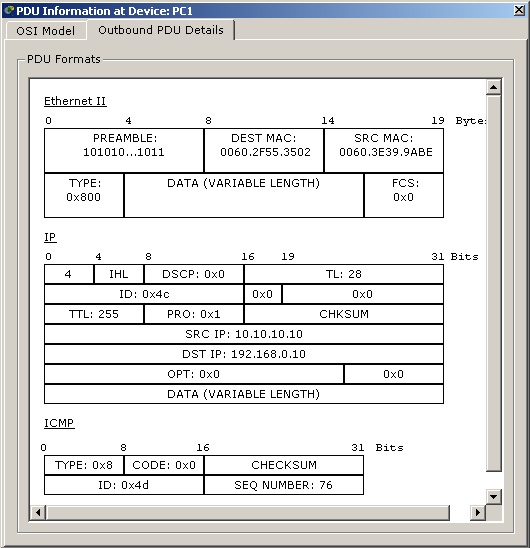
\includegraphics[width=0.4\textwidth]{tkinhalt/rsp_bilder/echoAnPc_detail.jpg}
  \caption{Detailansicht der ICMP Nachricht in PC1}
  \label{fig:detailEchoRequestPC1}
\end{figure}

\begin{figure}[htbp] 
  \centering
     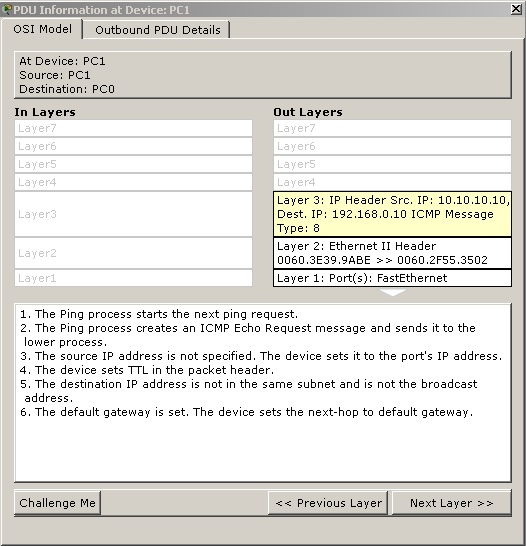
\includegraphics[width=0.5\textwidth]{tkinhalt/rsp_bilder/echoAnPc.jpg}
  \caption{Ansicht der ICMP Nachricht in PC1}
  \label{fig:EchoRequestPC1}
\end{figure}


\begin{figure}[htbp] 
  \centering
     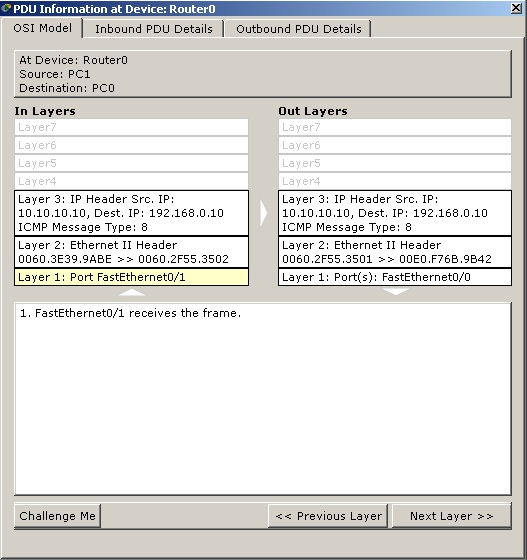
\includegraphics[width=0.5\textwidth]{tkinhalt/rsp_bilder/echoAnRouter.jpg}
  \caption{Ansicht der ICMP Nachricht im Router}
  \label{fig:EchoRequestRouter}
\end{figure}

\begin{figure}[htbp] 
  \centering
     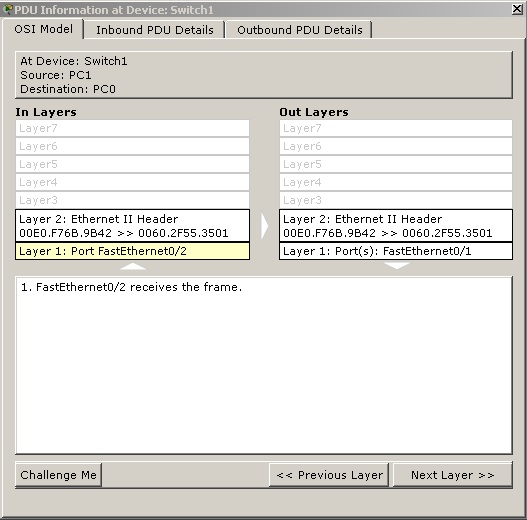
\includegraphics[width=0.5\textwidth]{tkinhalt/rsp_bilder/echoAnSwitch.jpg}
  \caption{Ansicht der ICMP Nachricht im Switch}
  \label{fig:EchoRequestSwitch}
\end{figure}

\begin{figure}[htbp] 
  \centering
     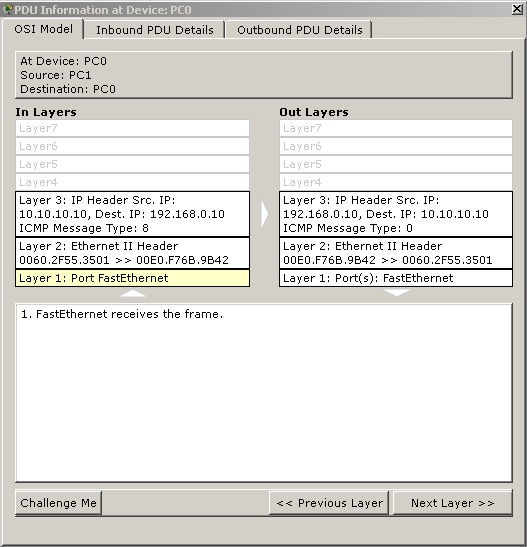
\includegraphics[width=0.5\textwidth]{tkinhalt/rsp_bilder/echoAnPcNULL.jpg}
  \caption{Ansicht der ICMP Nachricht im PC0}
  \label{fig:EchoRequestPCNULL}
\end{figure}


Der Weg des echo reply verl�uft analog zu dem Weg des echo request. Deswegen wird er nicht weiter beschrieben.


\subsection{Fazit}
Der Versuch mit Packet Tracer hat eine klare Verbindung zu fr�heren Vorlesungen hergestellt. Die Sachverhalte wurden bereits theoretisch vermittelt. Die Theorie wurde aber w�hrend des Versuchs sehr anschaulich dargestellt und letzte Unklarheiten wurden ausger�umt. 
%=========================================
% 	   Einleitung     		 =
%=========================================

\chapter{RSC Versuch}
\section{Einleitung}
Router und Switche begleiten uns im t�glichen Leben. Auch wenn sie oft nicht wahrgenommen werden, sind sie doch allgegenw�rtig. Ob mobiles Surfen, das Surfen am Computer oder auch telefonieren, diese T�tigkeiten sind ohne Router und Switche nicht m�glich. Der Netzwerkausr�ster Cisco rechnet bis zu Jahr 2018 mit einem weltweiten Internettraffic von 1,6 Zettabyte \cite{cisco_traffic_schaetzung}. 




%=========================================

%   Einleitung     =

%=========================================


\chapter{SDH Versuch}

\section{Allgemeine Beschreibung der Versuche}

%Kurze Einleitung ins Thema

Der folgende Versuch handelt von der Multiplextechnik SDH. SDH steht
Synchrone Digitale Hierarchie die es m�glich macht niederratige
Datenstr�me zu einem hochrratigen Datenstrom zu multiplexen, das Netz
taktet dabei vollkommen synchron. In unserem Versuchsaufbau werden wir
absichtlich verschiedene Fehler einspeisen sowie uns die
Pointeraktivit�ten im Netz genauer ansehen. Die M�glichkeit Fehler
einzuspeisen wird uns durch das Messger�t GN Elmi EST 2100 erm�glicht,
der ebenfalls als Multiplexer fungiert. Das Auswerten dieser Fehler
ist �ber die Software Telecommunications-Management-Network-Software
von Siemens gegeben. Der Rechner auf dem die Software l�uft ist �ber
die QST-E3 Schnittstelle mit den SMA 16 Multiplexern verbunden und
sammelt so die n�tigen Daten.

Die Multiplexer unter sich sind mit Lichtwellenleiter verbunden die
theoretisch eine Entfernung von gut 50Km schaffen w�rden. Da Elmi
leider nicht von Siemens ist, ist es auch nicht m�glich direkt �ber
die Software zu sehen wie Elmi sich als Multiplexer verh�lt.

\vspace{0.5 cm}
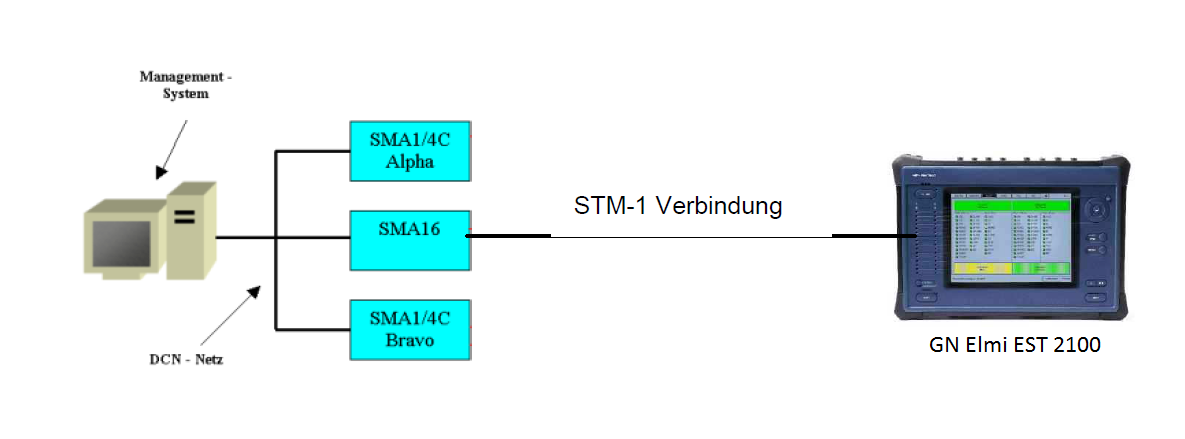
\includegraphics[width=1\textwidth]{tkinhalt/sdh/versuchsaufbau.png}\caption{Versuchsaufbau}\label{versuchsaufbau}
\vspace{0.5 cm}

\section{Versuchsgegenst�nde im Detail}

Im folgenden betrachten wir uns die TMNS und Elmi f�r das Verst�ndnis
den den Umgang etwas genauer.


\subsection{GN Elmi EST 2100}

Elmi ist ein Messger�t das direkt mit den anderen Multiplexern �ber
einen Lichtwellenleiter angeschlossen ist. Er fungiert in erster Linie
zum einspeisen von Fehlern ins Netz um zu betrachten wie sich das SDH
darauf verh�lt. Wie oben bereits erw�hnt ist er selbst ebenfalls Teil
des Netzes in Form von einem Multiplexers. Folgende Grafiken erl�utern
wie mit dem Ger�t um zu gehen ist.
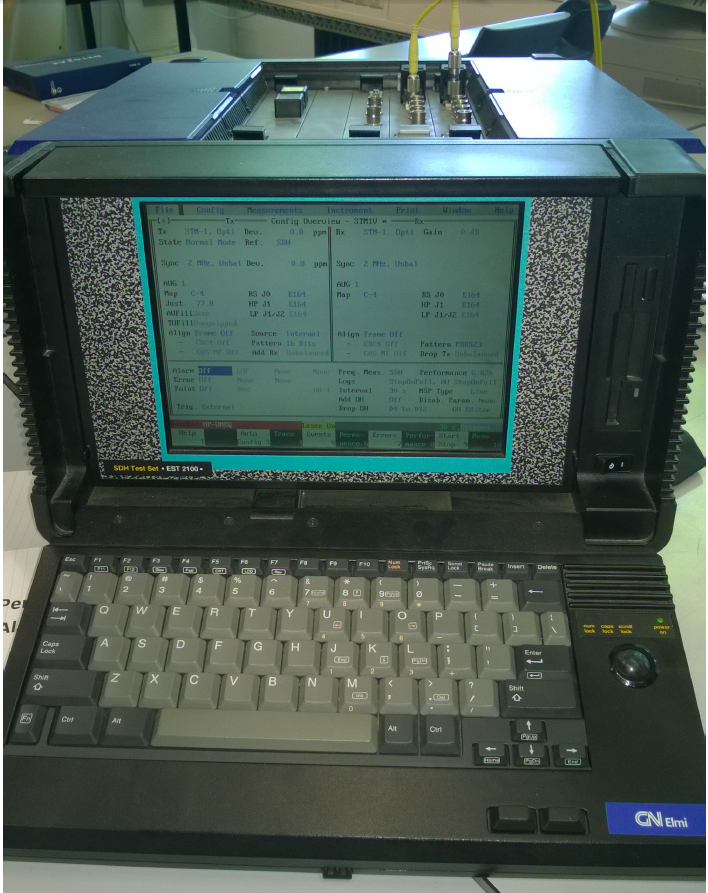
\includegraphics[width=1\textwidth]{tkinhalt/sdh/elmi_start.png}\caption{Startbildschirm GN Elmi EST 2100}\label{startbildschirm_elmi}
\vspace{0.5 cm}

Es gibt es veschiedene M�glichkeiten das Netz zu beeinflussen. Da Elmi
einen eigenen internen Systemtakt besitzt, kann man diesen auch
verwenden um so beispielsweise zwei verschiedene Takte im Netz zu
simulieren. Unter den Men�punkt Ref. kann man diesen dann
beeinflussen.


\todo{Bild von Taktmenu}


Desweiteren f�r unseren Versuch wichtige Funktion bietet die Sektion
ALARM. Hier kann man nach belieben Fehler ins Netz einspeisen. Diese
kann man entweder als Burst, das bedeutete �ber einen bestimmten
Zeitrahmen, oder kontinuierlich setzen. F�r unserem Versuch werden nur
diese zwei Sektionen ben�tigt deswegen wird hier nicht weiter auf die
Funktionalit�t von Elmi eingegangen.
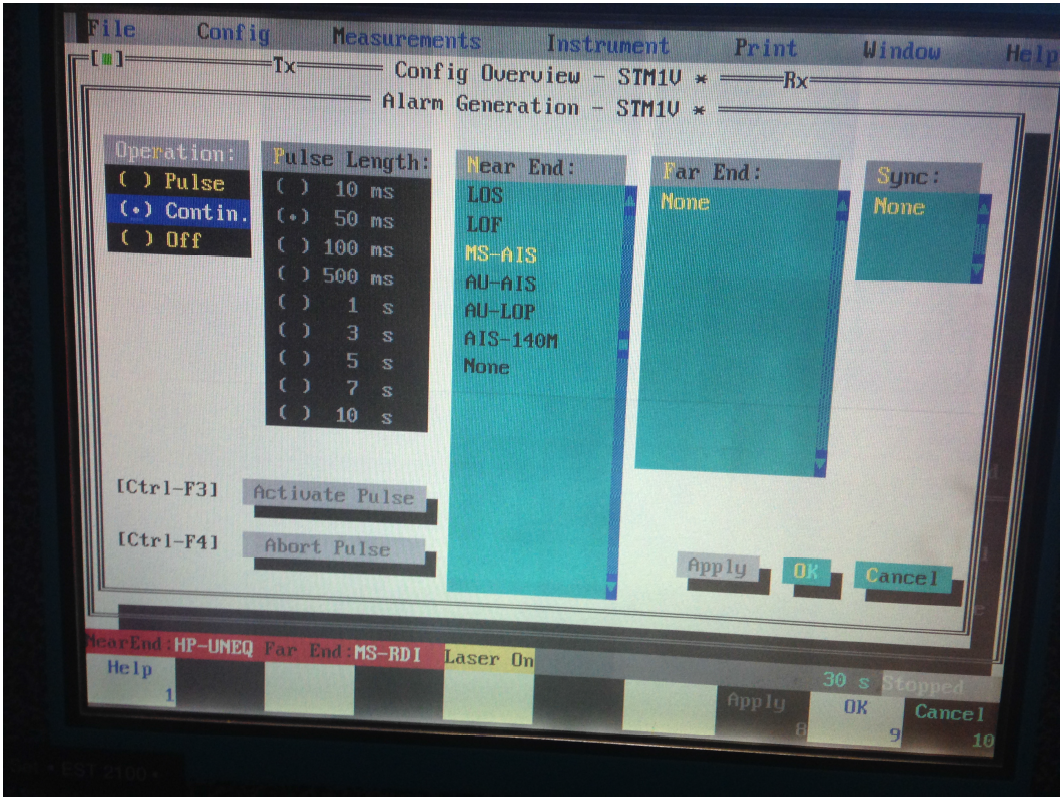
\includegraphics[width=0.9\textwidth]{tkinhalt/sdh/elmi_fehler.png}\caption{Fehlermenu GN Elmi EST 2100}\label{fehlermenu_elmi}
\vspace{0.5 cm}

\subsection{TMNS}

Die TMNS ist zur Analyse und �berwachung des SDH-Netzes hilfreich. In
der Hauptansicht wird das Netz abstrakt f�r eine gute �bersicht
dargestellt. Klickt man nun auf unser Testnetz \textit{K�ln}

auf die Performancemessung gelangt man in die f�r den Versuch
interessante Performanceansicht. \todo{stimmt das?}
\vspace{0.5 cm}
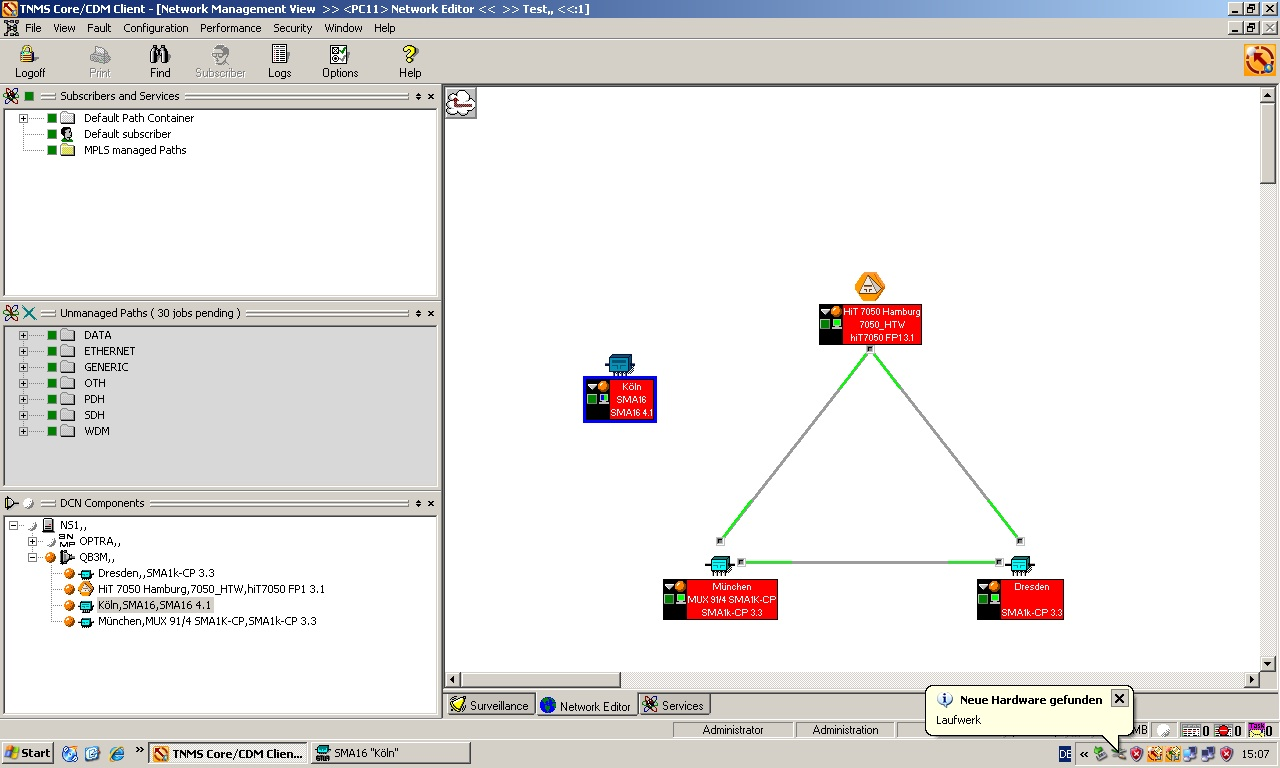
\includegraphics[width=0.9\textwidth]{tkinhalt/sdh/tnms.jpg}\caption{Telecommunications-Management-Network-Software}\label{TMNS}
\vspace{0.5 cm}

Im Hauptfenster werden s�mtliche Komponenten angezeigt die zu dem Netz
geh�ren bis auf Elmi. Hier werden bei einkommenden Fehlern, durch
rotes blinken markiert welche Komponente einen Fehler aufweist. In der
Folgenden Abbildung ist zu sehen wie die Komponente in dem Steckplatz
406 auf Port 3 einen einkommenden Fehler anzeigt. Port 1 und 2 sind
ebenfalls rot markiert jedoch weil die Ports konfiguriert sind aber
kein Kabel angeschlossen ist. Also k�nnen wir diese einfach
ignorieren.
\vspace{0.5 cm}
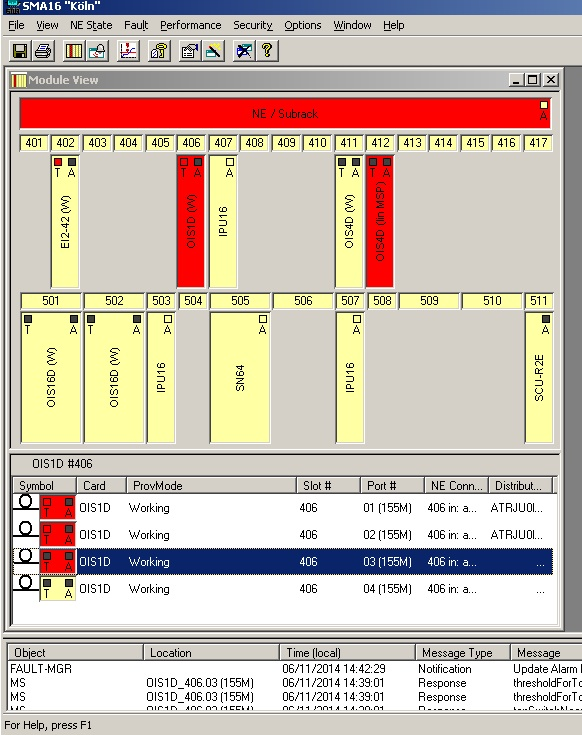
\includegraphics[width=0.9\textwidth]{tkinhalt/sdh/Fehler2.jpg}\caption{Einkommender Fehler im TMNS}\label{tms_incoming}
\vspace{0.5 cm}

Bei einem ankommenden Fehler kann man sich nun die Komponente genauer
anschauen indem man den entsprechenden Port sich unter die Lupe nimmt.
Durch Auswahl der Submenu-View gelangt man in eine Ansicht in der man
genauer sehen kann wo der Fehler entstanden ist.

\vspace{0.5 cm}
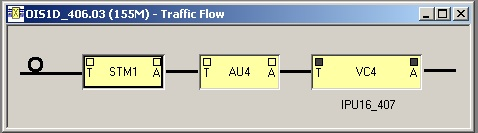
\includegraphics[width=0.9\textwidth]{tkinhalt/sdh/komponent-performance.jpg}\caption{Traffic Flow Fenster}\label{traficflow_fenster}
\vspace{0.5 cm}

Hier hat man nun je nach Fehler die Auswahl. Wenn es um Pointer geht
wird hier im Normalfall das AU-4 Fenster anfangen zu Blinken, wenn ein
Netz-Fehler auftritt das STM-1 Fenster.

Diese schauen wir uns hier noch im Detail an.

Zuerst sehen wir hier die Performance-Ansicht von dem AU-4 Fenster.

\vspace{0.5 cm}
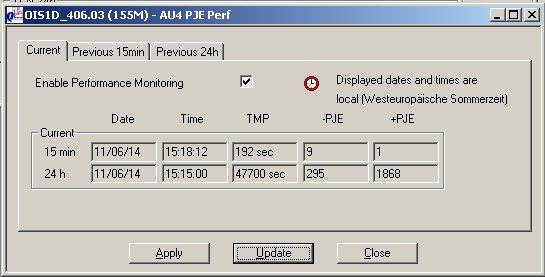
\includegraphics[width=0.9\textwidth]{tkinhalt/sdh/Pointerview_detail.jpg}\caption{Pointerview zur �berwachung der Aktivit�ten in AU4}\label{pointerview}
\vspace{0.5 cm}
%zur pointerview was schreiben

Dieses beinhaltet:


\begin{itemize}

\item Date - Das Aktuelle Datum

\item Time - Die Aktuelle Zeit

\item TMP - Dauer des gemessenen Intervalls

\item -PJE - Die gez�hlten Negativ Pointer-Vorg�nge

\item +PJE - Die gez�hlten Positiv Pointer-Vorg�nge

\end{itemize}


Die Aktualisierung der Daten findet nur manuell mit dem Update Knopf
statt. TMP ist hier im Auge zu behalten da die Daten alle 15 Minuten
in eine Log-Datei geschrieben werden. Die Log-Dateien sind in den
Reitern \textit{Previous 15min} und \textit{Previous 24h} wieder zu
finden.


Um im genau zu sehen was im STM-1 vor sich geht kann man sich hier
ebenfalls die Performance-Ansicht anzeigen lassen.

\vspace{0.5 cm}
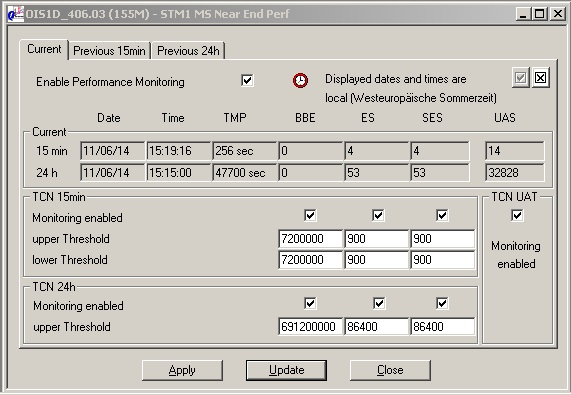
\includegraphics[width=0.9\textwidth]{tkinhalt/sdh/ms-near-end.jpg}\caption{STM1 Performance Fenster}\label{stm1_fenster}
\vspace{0.5 cm}

Folgende Daten werden angezeigt:


\begin{itemize}

\item Date - Das Aktuelle Datum

\item Time - Die Aktuelle Zeit

\item TMP - Dauer des gemessenen Intervalls

\item BBE - Background Block Error

\item ES - Errored Seconds

\item SES - Severely Errored Seconds

\item UAS - Unavailable Seconds

\end{itemize}


Was das Aktualisieren und das wegschreiben in die Log-Datei angeht ist
der Vorgang wie bereits vorher beschrieben der Fall.

Die Fehlerrate wird in Error-Sekunden angegeben die unterschiedliche
Aussagen �ber den Fehler angeben.


\begin{itemize}

\item ES - beinhaltet,innerhalb einer Sekunde, ein oder mehrere
fehlerhafte Bl�cke.

\item SES - beinhaltet, innerhalb einer Sekunde, 30 Prozent fehlerhafte Bl�cke.

\item UAS - Nach 11 SES gilt eine Leitung als nicht mehr verf�gbar. Im
Gegenzug gilt sie als verf�gbar, nach 11 Sekunden ohne SES.

\end{itemize}





\section{Fehlereinspeisung}

Nachdem wir alle f�r den Versuch erforderlichen Komponenten
kennengelernt haben, k�nnen wir nun den eigentlichen Versuch weiter
beschreiben. Im folgenden sollen drei verschiedene Fehlermeldungen mit
Hilfe von Elmi einmal kontinuierlich und einmal als Bursts eingespeist
werden. Wenn im empfangenen Signal Bitfehler enthalten sind sendet der
Empf�nger eine Alarm-Nachricht in Senderichtung zur�ck. Bei dieser
R�ckmeldung spricht man von REI (Remote Error Indication). Die f�r uns
wichtigen sind:


\begin{itemize}

\item LOS - Lost of Singnal, R�ckgang der eingehenden optischen
Leistungspegel, verursacht hohe Bitfehlerrate

\item MS-AIS - Multiplex Section Alarm Indication Signal, wird
ausgel�st wenn K2 (bits 6, 7, 8) auf 111 gesetzt ist f�r mehr als 3
Frames.

\item LOF - Lost of Frame tritt auf wenn das Signal f�r mehr als 3 ms
OOF (Out of Frame) ist.

\item OOF - Out of Frame tritt auf wenn die Bytes A1 und A2 l�nger als
624 $\mu$ s  fehlerhaft sind 
\end{itemize}


Sind im empfangenen Signal Bitfehler enthalten, meldet der Sensor

BIP Errors. Da das nicht gleichbedeutend mit dem Ausfall der Verbindung

ist, spricht man von einer Anomalie, die in Senderichtung zur�ckgemeldet

wird. Die R�ckmeldung wird als REI (Remote Error Indication)

bezeichnet.




\subsubsection{Kontinuierliches Fehlereinspeisen}

Zuerst werden wir die Fehler kontinuierlich einspeisen. Nach dem
feuern der Fehler f�ngt die entsprechende Komponente an zu Blinken und
wir klicken uns bis in das STM-1\_performance-Fenster durch.

\vspace{0.5 cm}
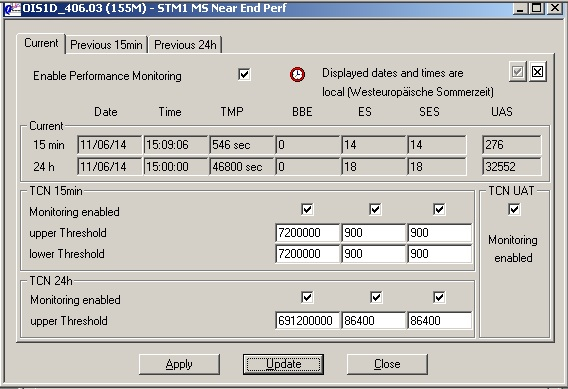
\includegraphics[width=0.9\textwidth]{tkinhalt/sdh/stm1-konti.jpg}\caption{STM1 Performance Fenster mit hoher UAS-Rate}\label{stm1_hohe_uas}
\vspace{0.5 cm}

Die Ergebnisse sind alle wie zu erwarten gleich. Alle drei
Fehlermeldungen lassen den UAS-Counter solange ansteigen bis man
aufh�rt den Fehler einzuspeisen. Da alle drei Fehler kontinuierlich
auftreten verursachen sie dauerhaft SES und somit nach kurzer Zeit
UAS. Somit sind kontinuierliche Fehler sehr schwerwiegend und sofort
zu behandeln.

Hier noch einmal ein Tabellarischer �berblick �ber alle gemessenen Daten:


\begin{table}
\begin{tabular}{|*{6}{c|}}
\hline
Fehlermeldung & Burst-Time & ES & SES & UAS & Fenster \\
\hline
\hline
MS-AIS & Kontinuierlich & 0 & 0 & ++ & STM1 \\
\hline
LOS & Kontinuierlich & 0 & 0 & ++ & STM1 \\
\hline
LOF & Kontinuierlich & 0 & 0 & ++ & STM1 \\
\hline
\end{tabular}
\centering
\caption{Kontinuierliches steigen der UAS solange die Fehlermeldung eingespeist wird}
\end{table}
\subsubsection{Burst Fehlereinspeisung}


Als zweites Verursachen wir eine MS-AIS und ein LOS jeweils innerhalb
von 100ms, einer Sekunde, und sieben Sekunden.

\begin{table}
\begin{tabular}{|*{6}{c|}} 
\hline 
Fehlermeldung & Burst-Time & ES & SES & UAS & Fenster \\
\hline 
\hline 
MS-AIS & 100 ms & 1 & 1 & 0 &STM1 \\
\hline 
MS-AIS & 1 s & 2 & 2 & 0 & STM1 \\
\hline 
MS-AIS & 7 s & 8 & 8 & 0 & STM1 \\
\hline 
LOS & 100 ms & 3 & 3 & 0 & STM1 \\
\hline 
LOS & 1 s & 4 & 4 & 0 & STM1 \\
\hline 
LOS & 7 s & 0 & 0 & 14 & STM1 \\
\hline 
\end{tabular}
\centering
\caption{Konsequenzen auf verschieden lange Fehlermeldungen}
\end{table}
\vspace{1 cm}

Wie man anhand der Tabelle sehen kann l�st die MS-AIS lediglich
maximal 8 SES aus und somit wird die Leitung nicht als Unavailable
gesetzt.

Zu Beobachten war das bei den kruzen Bursts die TMNS �berhaupt gar
nicht auf den Fehler reagiert. Das ist erkl�rbar da bevor der Fehler
erkannt wird, er bereits wieder vorbei ist. Bei den LOS Alarmen sind
die Error Sekunden schon betrachtlich h�her. Ein sieben Sekunden
langer LOS kann die Leitung bereits f�r einige Momente ausser gefecht
setzen wie man an dem UAS Feld erkennen kann.


\subsection{Pointer}

Da das SDH-Netz ein voll getaktetes Netz ist und so durch
Taktunterschiede es theoretisch zu einer �berlast kommen kann, gibt es
Pointer. Dieser ist in der Administrative Unit zu finden und zeigt auf
die Position der Nutzinfomrationen im Payload Bereich. Durch Pointer
ist es m�glich die Taktunterschiede, durch einf�gen von Leer-Bytes
oder fr�heres Senden von Payload, auszugleichen. Es k�nnen allerdings
nur in jedem vierten Rahmen nach Ank�ndigung die Pointer angepasst
werden.

In diesem Versuch besch�ftigen wir uns mit dem dekrementieren und
Inkrementieren von Pointern. Zus�tlich dazu, werden wir mit dem
Systemtakt des Netzes hantieren.


\subsubsection{Manuelles negativ und positiv Justieren}

Elmi hat f�r die Justierung des Pointers ein eigenes Menu. Hier kann
man einstellen ob man die Pointer-Justierung dauerhaft alle 1500 ms
oder manuell durchf�hren will.


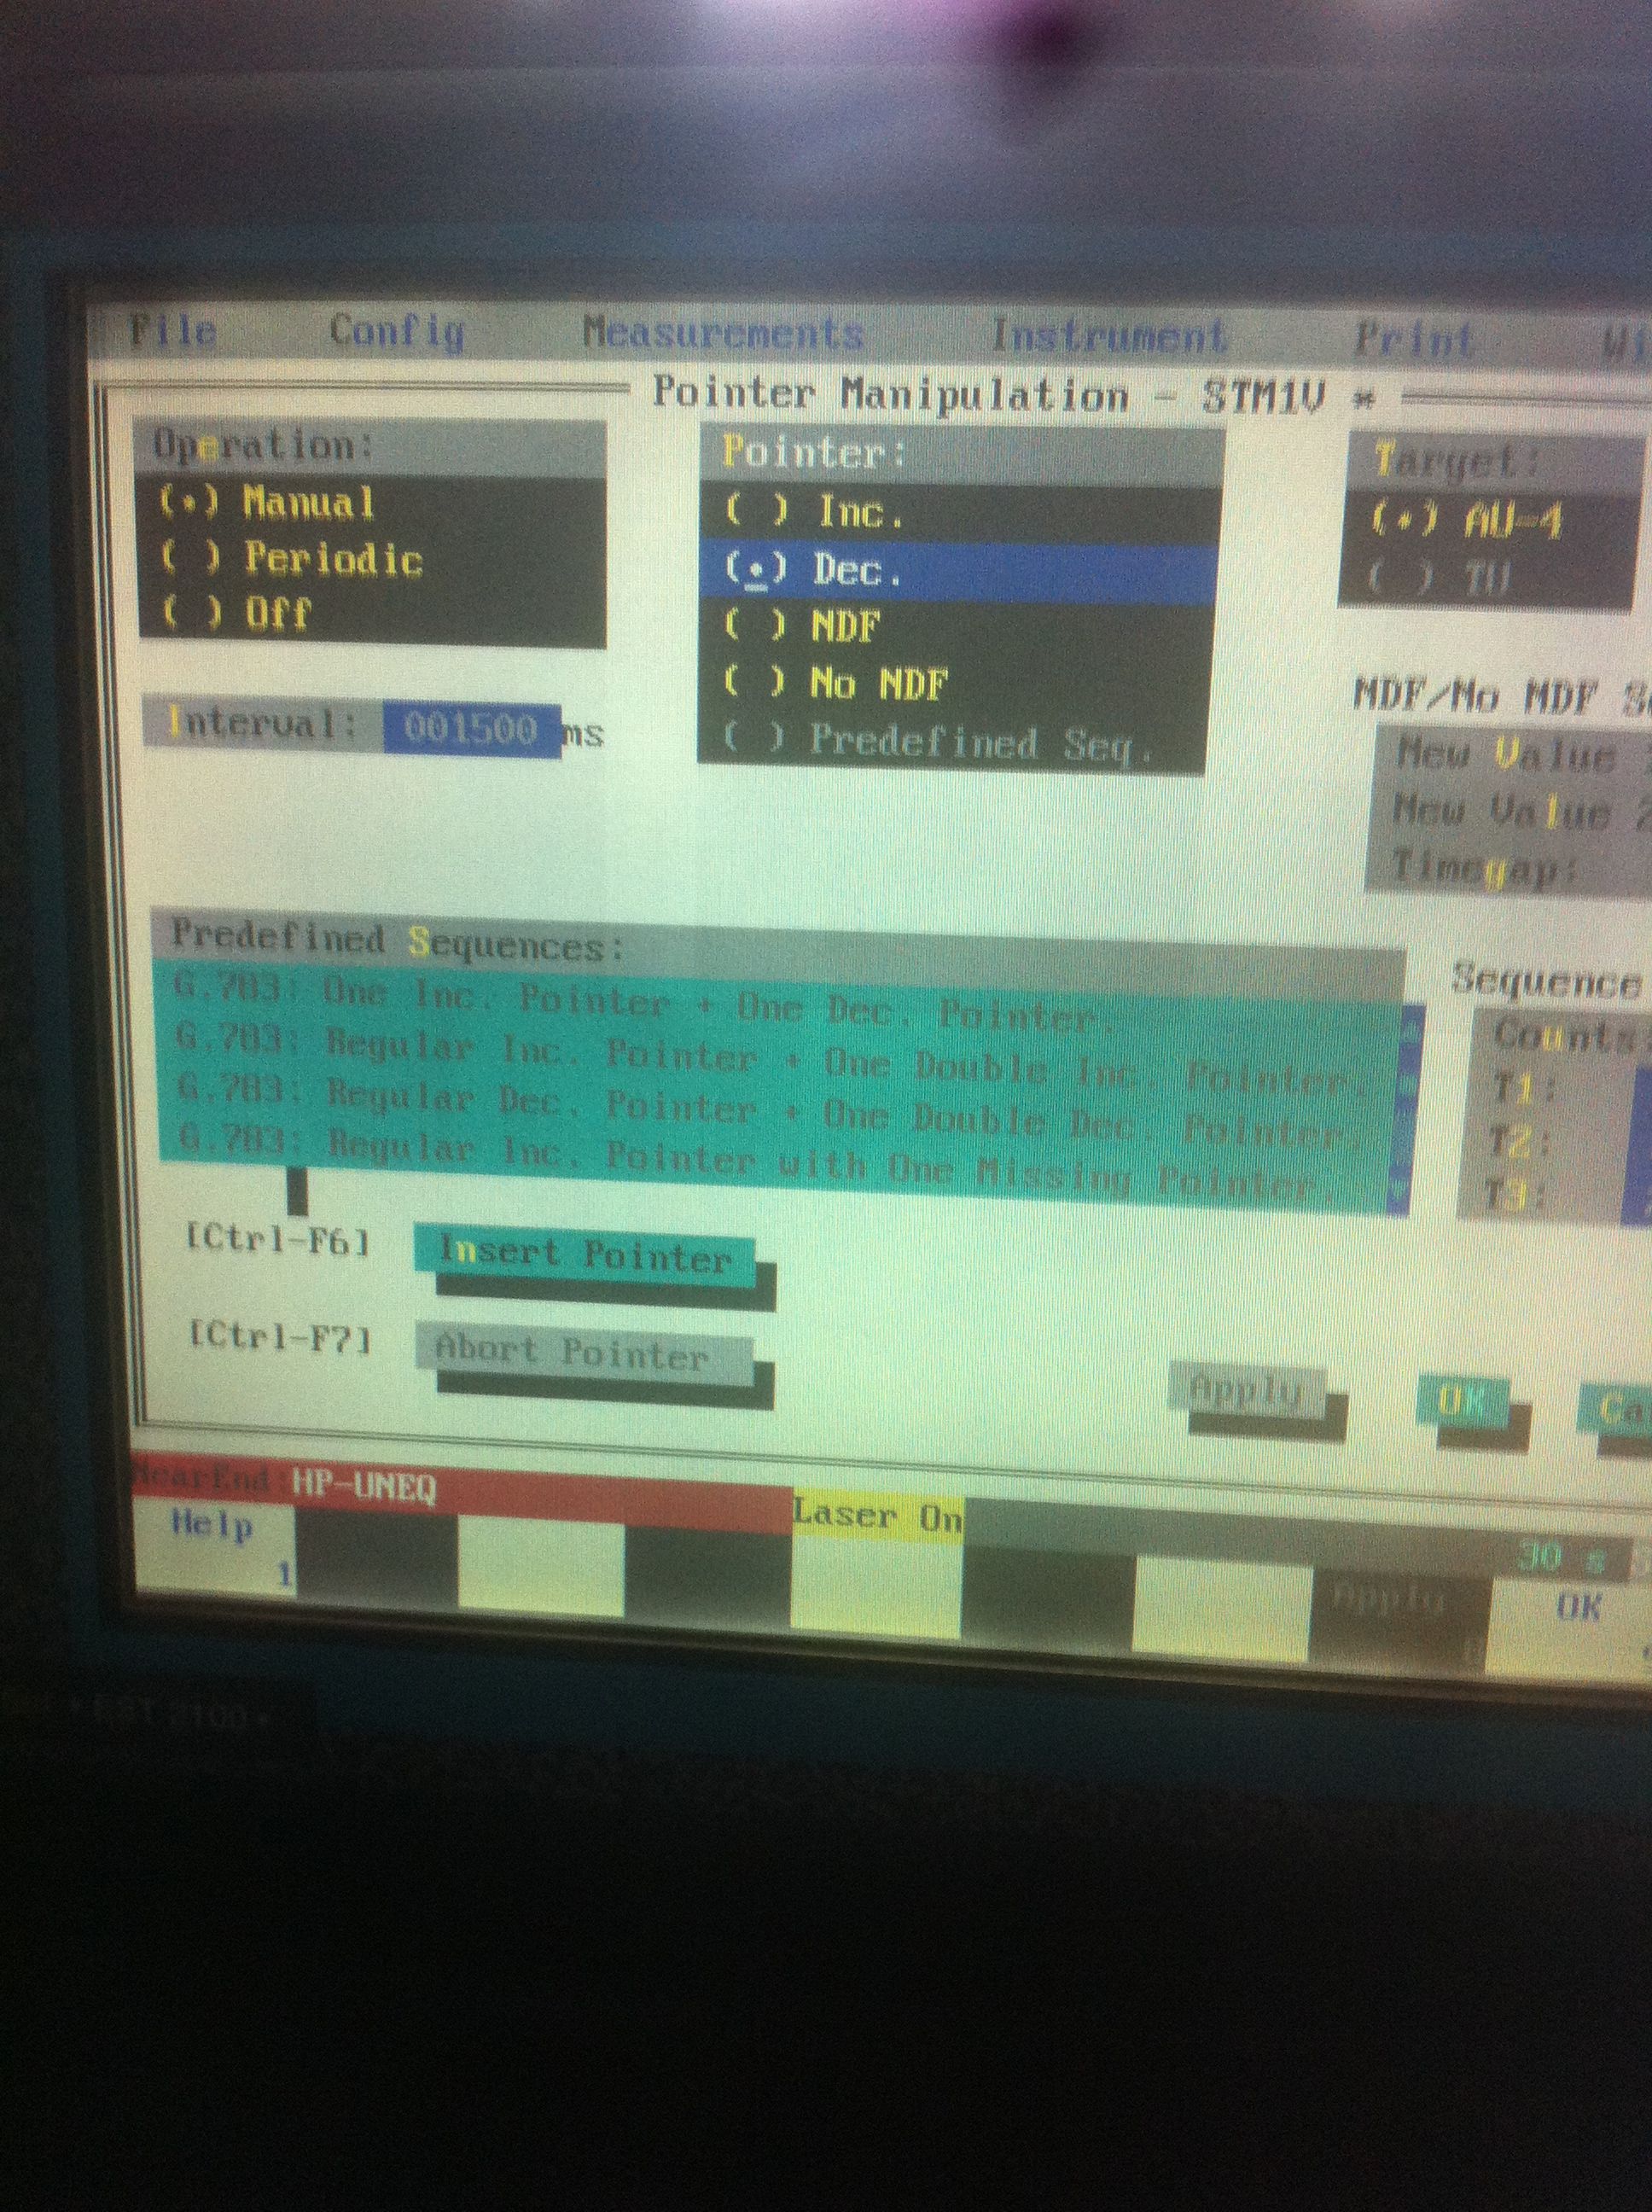
\includegraphics[width=0.9\textwidth]{tkinhalt/sdh/IMG_1937.JPG}\caption{Dekrementieren des Pointers}\label{dekrement_pointer}
\vspace{0.5 cm}

Zuerst Dekrementieren wir den Pointer was ein Pointer Justification
Event ausl�st und in TMNS im Performance Menu von AU-4 als
-PJE-Erh�hung wahrzunehmen ist.

Entsprechend umgekehrt verh�lt sich das System f�r die Inkrementierung
des Pointers. Im Versuch war zu erkennen das die ersten drei
gesendeten Werte nicht in dem Perfomance-Fenster sichtbar waren. Dies
ist darauf zur�ck zu f�hren das nur bei jedem vierten Rahmen eine
Pointer-Aktivit�t durchgef�hrt wird. Also wurden die ersten drei als
Ank�ndigung verstanden das nun der Pointer ge�ndert wird. \todo{stimmt
das denn auch?}


\subsubsection{�ndern des Taktes von Elmi}

�ndert man den Takt von Elmi auf den Internen so kann man einen hohen
Sprung des +PJE Feldes beobachten. Dies zeigt das das System die
beiden Multiplexer versucht zu synchronisieren. Dannach sieht man das
das +PJE Feld weiter steigt, um etwa drei pro Sekunde. Die Erkl�rung
daf�r ist, das der interne Takt von Elmi etwas langsamer ist als der
des anderen Multiplexern. So muss dieser positiv Inkrementieren um den
Takt auszugleichen und das Netz synchron zu halten.


\subsubsection{kontinuierliches negatives Justieren bei Internem Takt}

Als letztes m�chten wir gerne noch Versuchen was passiert wenn wir
zus�tzlich zu dem ge�ndertem Takt noch negativ den Pointer justieren.
Bei verwendung des internen Taktes von Elmi haben wir festgestellt das
eine positive Pointerjustierung n�tig ist um das Netz Synchron zu
halten. Wenn wir nun aber auf der Sende Seite den langsameren Takt
durch negativ Justierung ausgleichen kann man beobachten wie die
ben�tigten Pointer-Aktivit�ten sinken. Wenn man das Intervall
entsprechend weit runter stellen w�rde k�nnte man den kompletten
ausgleich zwischen den unterschiedlichen Takten erreichen. In dem
Versuch haben wir beobachtet wie sich die Pointerjustierung auswirkt.
Dies ist hier noch einmal Tabellarsich aufgef�hrt.

\vspace{1 cm}
\begin{table}
\begin{tabular}{|*{2}{c|}}
\hline
Justierung & PointerAktivit�t \\
\hline
Inkrementierung & 5 Pointer pro Sekunde\\
\hline
Dekrementierung & 3 Pointer pro Sekunde \\
\hline
Ohne & 4 Pointer pro Sekunde \\
\hline
\end{tabular}
\centering
\caption{�nderungen der Pointeraktivit�ten bei internem Takt}
\end{table}
\vspace{1 cm}

Die Tabelle zeigt auf das mit einer Positiven Justierung des Pointers
zus�tlich zu dem unteschiedlichen Takt eine noch h�here
Pointer-Aktivit�t n�tig ist um das System synchron zu halten. Wie oben
beschreiben f�hrt eine Dekrementierung zu einem ann�herndem Ausgleich.
Diese Aussage wird unterst�tzt wenn man sich die Spalte Ohne
Justierung ansieht. Hier ist es etwa der Mittelwert der beiden
anderen.


\section{Fazit}

In den Versuchen wurde das bereits erlangte Wissen praktisch
angewandt. Vor allem in dem Bereichen Pointer wurden die das
Verst�ndnis daf�r sehr viel klarer und die Zusammenh�nge eindeutiger.
Allerdings waren die Versuche alle sehr klar definiert und die
Erwartungen nicht �berrascht.
%=========================================
% 	   Einleitung     		 =
%=========================================
\chapter{RN Versuch}
\section{Versuchsaufbau}
Der Aufbau des Versuchs besteht aus zwei Routern, einem Switch, zwei Host Rechnern und den entsprechenden Kabeln. Vor Beginn des Versuchs werden sowohl die Switche, als auch die Router auf ihre Werkseinstellungen zur�ck gesetzt. Damit wird sichergestellt, dass eventuelle Konfigurationen aus vorangegangen Versuchen gel�scht werden und keine Fehler verursachen.

Nachdem die Hardware vorbereitet ist, werden die Adressen aus einem gegebenen Netz errechnet. Gegeben ist das Netz 192.168.1.0/24. Dieses soll in ein Netz mit max. 120 Hosts und ein Netz mit max.  60 Hosts aufgeteilt werden. Das gr��ere Netz soll mit dem Router R1 verbunden werden, das Kleinere soll mit dem Router R2 verbunden werden. Da die Router sich in dieser Konfiguration in verschiedenen Netzen befinden, muss noch ein Transfernetz eingerichtet werden, damit sie untereinander kommunizieren k�nnen. Aus diesen Anforderungen ergeben sich die drei Netze, die in der Tabelle \ref{tab:berechneteNetzwerke}.

\begin{table}[h]
\begin{tabular}{|*{2}{c|} p{0.15\linewidth}|*{3}{c|}}
\hline
Netzadresse & BC & Hosts & Subnet Mask & Slash & Adressen\\
\hline
\hline
192.168.0.1 & 192.168.1.127 & 192.168.1.1 - 192.168.1.126 & 255.255.255.128 & /25 & 126 \\
\hline
192.168.0.128 & 192.168.1.191 & 192.168.1.129 - 192.168.1.190 & 255.255.255.192 & /26 &62 \\
\hline
192.168.0.192 & 192.168.1.199 & 192.168.1.193 - 192.168.1.198 & 255.255.255.248 & /29 &6	 \\
\hline
\end{tabular}
\caption{Die berechneten Netzwerke}
\label{tab:berechneteNetzwerke}
\end{table}

Nach dieser Berechnung kann eine �bersicht aufgestellt werden, wie das Netzwerk aufgebaut werden soll. Die Adressvergabe ist in Tabelle \ref{tab:berechneteNetzwerke} dargestellt.
\begin{table}[H]
\begin{tabular}{|*{5}{c|}}
\hline
Device & Host Name & Interface & IP Address & Subnet Mask \\
\hline
R1 & R1 & Serial 0/0/0(DCE) & 192.168.1.193 & 255.255.255.248 \\
\hline
& & FE 0/0 & 192.168.1.1 & 255.255.255.128 \\
\hline
H1 &H1 &  Ethernet & 192.168.1.2 & 255.255.255.128 \\
\hline
H2 & H2 & Ethernet & 192.168.1.130 & 255.255.255.192 \\
\hline
R2 & R2 & Serial 0/0/0(DTE) & 192.168.1.194 &255.255.255.248 \\
\hline
& & FE 0/0 & 192.168.1.129 & 255.255.255.192\\
\hline
\end{tabular}
\caption{Der Aufbau des Netzwerks}
\label{tab:aufbauNetzwerk}
\end{table}


\begin{figure}[H] 
  \centering
     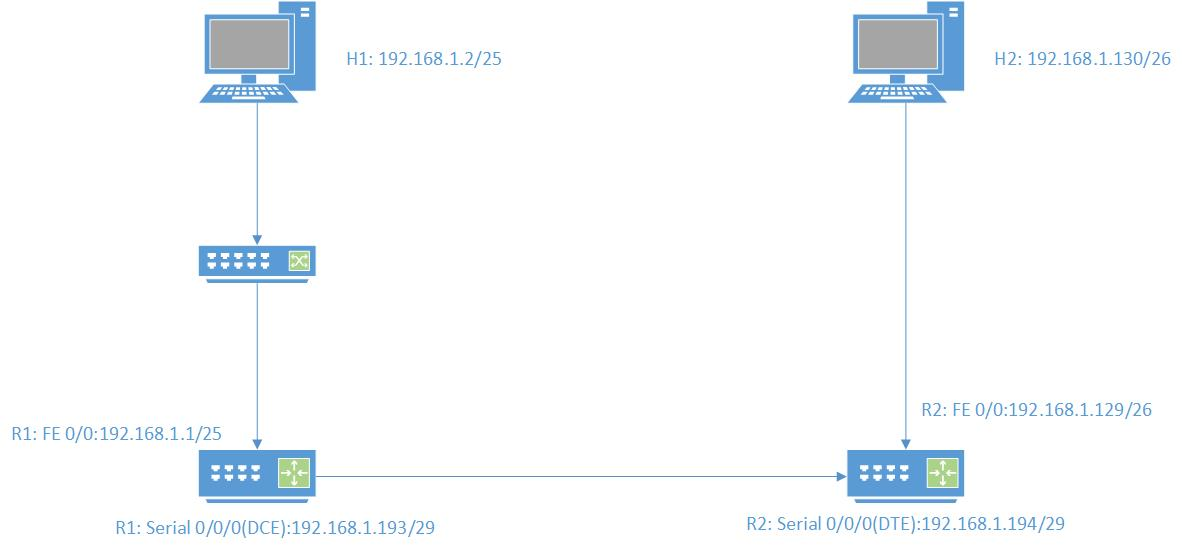
\includegraphics[width=1\textwidth]{tkinhalt/rn_bilder/rn.jpg}
  \caption{Der Aufbau unseres Netzwerks}
  \label{fig:aufbauNW}
\end{figure}
\todo{H1 h�ngt glaube ich an R1 und H2 h�ngt an R2}
Nachdem die Netze berechnet sind werden sowohl Router als auch Hosts entsprechend eingerichtet.

\section{Routing}
\subsection{�berpr�fung der Routingeinstellungen}
Der Befehl \textit{show ip route} zeigt die Routen an, die der Router gespeichert hat.
\begin{lstlisting}[captionpos=b,caption=Die Routing Table von R1]
R1#show ip route
Codes: C - connected, S - static, R - RIP, M - mobile, B - BGP
       D - EIGRP, EX - EIGRP external, O - OSPF, IA - OSPF inter area 
       N1 - OSPF NSSA external type 1, N2 - OSPF NSSA external type 2
       E1 - OSPF external type 1, E2 - OSPF external type 2
       i - IS-IS, su - IS-IS summary, L1 - IS-IS level-1, L2 - IS-IS level-2
       ia - IS-IS inter area, * - candidate default, U - per-user static route
       o - ODR, P - periodic downloaded static route

Gateway of last resort is not set

     192.168.1.0/24 is variably subnetted, 2 subnets, 2 masks
C       192.168.1.0/25 is directly connected, FastEthernet0/0
C       192.168.1.192/29 is directly connected, Serial0/0/0
\end{lstlisting}

\begin{lstlisting}[captionpos=b,caption=Die Routing Table von R2]
R2#show ip route
Codes: L - local, C - connected, S - static, R - RIP, M - mobile, B - BGP
       D - EIGRP, EX - EIGRP external, O - OSPF, IA - OSPF inter area
       N1 - OSPF NSSA external type 1, N2 - OSPF NSSA external type 2
       E1 - OSPF external type 1, E2 - OSPF external type 2
       i - IS-IS, su - IS-IS summary, L1 - IS-IS level-1, L2 - IS-IS level-2
       ia - IS-IS inter area, * - candidate default, U - per-user static route
       o - ODR, P - periodic downloaded static route, + - replicated route

Gateway of last resort is not set

      192.168.1.0/24 is variably subnetted, 4 subnets, 3 masks
C        192.168.1.128/26 is directly connected, FastEthernet0/0
L        192.168.1.129/32 is directly connected, FastEthernet0/0
C        192.168.1.192/29 is directly connected, Serial0/0/0
L        192.168.1.194/32 is directly connected, Serial0/0/0
\end{lstlisting}

Der Router hat keine Route in das Netzwerk 192.168.1.128. Dieses Netzwerk kann er nicht direkt erreichen und eingestellt ist auch keine.

Ob die beiden Router eine Verbindung zueinander haben kann mit einem Ping getestet werden:
\begin{lstlisting}[captionpos=b,caption=Ping von R1 zu R2]
R1#ping 192.168.1.129

Type escape sequence to abort.
Sending 5, 100-byte ICMP Echos to 192.168.1.129, timeout is 2 seconds:
.....
Success rate is 0 percent (0/5)
\end{lstlisting}


Dieser Ping war nicht erfolgreich.

Ein Ping wird auch von H1 zu H2 ausgef�hrt. Dieser Ping ist auch nicht erfolgreich.

Dass beide Pings nicht erfolgreich waren liegt daran, dass sich die die Router, bzw. die Pc je in unterschiedlichen Netzwerken befunden haben. Da noch keine Routen konfiguriert waren, konnten die Router die Datenpakete nicht weiterleiten.

\subsection{Einstellen des Routingprotokolls}
RIP ist ein Interieur Gateway Protokoll, also ein Routing Protokoll, das innerhalb eines autonomen Netzes benutzt wird. Dieses Protokoll ist in der Lage eine eigene Routingtabelle aufzubauen. Dadurch bleibt das Netzwerk flexibel und muss beim Einbau von neuen Ger�ten nicht neu konfiguriert werden. Da wird in unserem Netzwerk verschiedene und klassenlose Netzmasken nutzen m�ssen wir RIP v2 nutzen.
Der Befehl \textit{router rip} aktiviert das RIP routing und versetzt den Router in den Konfigurationsmodus. Mit dem Befehl \textit{version 2} konfiguriert man die Software dass sie nur noch RIP v2 Pakete empf�ngt und aussendet. Der Befehl \textit{network 192.168.1.0} wei�t dem Netzwerk 192.168.1.0 das Routing Protokoll zu. Der Router 1 wird mit der Befehlssequenz
\begin{lstlisting}[captionpos=b,caption=Befehlssequenz zum Konfigurieren von R1]
R1(config)#router rip 
R1(config-router)# version 2 
R1(config-router)# network 192.168.1.0
R1# copy running-config startup-config
\end{lstlisting} zum Routen eingerichtet. Die letzte Zeile speichert die neuen Einstellungen in den NVRAM.

R2 wird analog konfiguriert.

\subsection{�berpr�fen der Routing Einstellungen}
Nach dem Einstellen der Routing Konfiguration kann diese wieder �berpr�ft werden. 

\begin{lstlisting}[captionpos=b,caption=Die Ausgabe der Routingseinstellungen von R1]
R1#show ip route 
Codes: C - connected, S - static, R - RIP, M - mobile, B - BGP
       D - EIGRP, EX - EIGRP external, O - OSPF, IA - OSPF inter area 
       N1 - OSPF NSSA external type 1, N2 - OSPF NSSA external type 2
       E1 - OSPF external type 1, E2 - OSPF external type 2
       i - IS-IS, su - IS-IS summary, L1 - IS-IS level-1, L2 - IS-IS level-2
       ia - IS-IS inter area, * - candidate default, U - per-user static route
       o - ODR, P - periodic downloaded static route

Gateway of last resort is not set

     192.168.1.0/24 is variably subnetted, 3 subnets, 3 masks
C       192.168.1.0/25 is directly connected, FastEthernet0/0
C       192.168.1.192/29 is directly connected, Serial0/0/0
R       192.168.1.128/26 [120/1] via 192.168.1.194, 00:00:20, Serial0/0/0
\end{lstlisting}

In der Routingtabelle werden die Netzwerke 192.168.1.0/25 , 192.168.1.192/29 und 192.168.1.128/26 angezeigt. Das \glqq R\grqq~bedeutet, dass dieses Netzwerk �ber RIP, also durch Routing erreicht werden kann. \glqq via 192.168.1.194\grqq~bedeutet, dass diese Adresse  �ber die Adresse 192.168.1.194 erreicht werden kann. Diese Adresse ist dann das Gateway um in das Netz 192.168.1.128 zu erreichen. Serial 0/0/0 gibt an, �ber welchen Port des Routers das Netzwerk erreicht werden kann.


\begin{lstlisting}[captionpos=b,caption=Die Ausgabe der Routingseinstellungen von R2]
R2#show ip route
...

      192.168.1.0/24 is variably subnetted, 5 subnets, 4 masks
R        192.168.1.0/25 [120/1] via 192.168.1.193, 00:01:14, Serial0/0/0
C        192.168.1.128/26 is directly connected, FastEthernet0/0
L        192.168.1.129/32 is directly connected, FastEthernet0/0
C        192.168.1.192/29 is directly connected, Serial0/0/0
L        192.168.1.194/32 is directly connected, Serial0/0/0
\end{lstlisting}

In der Routingtabelle von R2 sind die Netzwerke 192.168.1.0, 192.168.1.128 und 192.168.1.192 aufgef�hrt. 

Ob die Routingeinstellungen tats�chlich funktionieren, kann wieder mit Pings getestet werden. Dieses Mal sind die Pings erfolgreich. Der Grund ist, dass die Router nun ein Routingprotokoll konfiguriert und Informationen haben, wie sie das jeweils andere Interface erreichen. 

\subsection{�berpr�fung der RIP Kommunikation}
\begin{lstlisting}
*Jun 18 12:27:33.923: RIP: build update entries
*Jun 18 12:27:33.923:   192.168.1.128/26 via 0.0.0.0, metric 2, tag 0
*Jun 18 12:27:33.923:   192.168.1.192/29 via 0.0.0.0, metric 1, tag 0
\end{lstlisting}
Der Befehl \textit{debug ip rip} aktiviert die Ausgabe der Rip Kommunikation eines Routers. Mit diesem Befehl kann mitgelesen werden, welche Informationen zwischen den Routern ausgeteilt werden. Auff�llig ist, dass alle RIP Informationen �ber das Interface 0.0.0.0 geschickt werden. Diese Adresse bezeichnet das Defaultgateway, bzw. alle Netze, die unbekannt sind werden mit dieser Adresse belegt.

Was noch auff�llt ist, dass die Netze unterschiedliche Metriken haben. Die unterschiedlichen Metriken ergeben sich aus der Route, die gew�hlt werden muss. Das Netzwerk 192.168.1.192/29 kann direkt vom Router R1 erreicht werden. Um das Netzwerk 192.168.1.128/26  zu erreichen muss der Router den Umweg �ber das Netzwerk 192.168.1.192 nehmen. Die Metrik von Rip v2 sagt aus, wie viele Hops eine Route hat.
Da wir uns beim einteilen des Netzwerkes zwischen den 2 Routern vertan haben, statt /30 haben wir /29 benutzt, kann es zu Abweichungen zur Aufgabenstellung kommen. Erinnern wir uns an die Grafik \ref{fig:aufbauNW} wird schnell klar, warum die Routen unterschiedliche Metriken haben.

\subsection{Reflection}
a. What would happen to the routing table on router R1 if the Ethernet network on router R2 went down? Configure this case and analyze.
If the routing table on R2 went down, R2 was unable to reach it's connected networks. The PC were unable to reach each other. Also H2 was unable to reach R1. R1 would change it's metric for the network 192.168.1.129 to 16 (not reachable).
\todo{Auch erfunden}


b. What would happen if router R1 was configured to run RIPv1, and R2 was configured to run RIPv2? Configure this case and analyze with show ip route and debug ip rip.

R1 would ignore all sent RIP v2 information and send out RIP v1 information.
\begin{lstlisting}
*Jun 18 12:33:51.091: RIP: ignored v2 packet from 192.168.1.194 (illegal version)
*Jun 18 12:33:55.343: RIP: sending v1 update to 255.255.255.255 via FastEthernet0/0 (192.168.1.1)
\end{lstlisting}


%********************************************************************
% Other Stuff in the Back
%*******************************************************
\cleardoublepage%********************************************************************
% Bibliography
%*******************************************************
\printbibliography

% ********************************************************************
% Appendix/Anhang
%***************************************************************
\appendix

%*******************************************************
\cleardoublepage\pagestyle{empty}

\hfill

\vfill

\pdfbookmark[0]{Kolophon}{colophon}
\section*{Kolophon}
Dieses Dokument wurde mit der \LaTeX-Vorlage f�r Abschlussarbeiten an der htw saar im Bereich Informatik/Mechatronik-Sensortechnik erstellt (\currentVersion). Die Vorlage wurde von Yves Hary und Andr\'e Miede entwickelt (mit freundlicher Unterst�tzung von Thomas Kretschmer und Helmut G. Folz).


\end{document}
% ********************************************************************
